\documentclass[10pt,a4paper]{article}
\usepackage[utf8]{inputenc}
\usepackage[T1]{fontenc}
\usepackage{lmodern}
\usepackage[margin=1.75cm]{geometry}
\usepackage{amsmath,amssymb,amsfonts}
\usepackage{booktabs}
\usepackage{graphicx}
\graphicspath{{../figures/}}
\usepackage{float}
\usepackage[section]{placeins}
\usepackage{hyperref}
\usepackage{xcolor}
\usepackage{caption}

\hypersetup{
    colorlinks=true,
    linkcolor=blue!60!black,
    citecolor=blue!60!black,
    urlcolor=blue!60!black
}

\title{Safe and Smooth Automatic Train Speed Control:\\
From State-Augmented MPC to Multi-Station Hierarchical\\
Differential and Assume-Guarantee Contract Shielding}
\author{Technical Report}
\date{\today}

\begin{document}
\maketitle

\begin{abstract}
Modern railway automation splits longitudinal train control into two disconnected layers: Automatic Train Protection (ATP), which guarantees safety through conservative worst-case braking envelopes and rigid speed ceilings, and Automatic Train Operation (ATO), which seeks comfortable acceleration profiles, low traction energy, punctual station arrivals, and accurate platform docking without formal multi-property guarantees. Our objective is to merge ATP safety certification and ATO multi-objective trajectory optimization within a single real-time closed-loop architecture guarded by runtime safety shielding, while cleanly separating fixed physical comfort specifications from genuinely learned and online-estimated components. We develop this framework through four sequential stages. First, we model the nonlinear longitudinal train dynamics—including temperature-dependent aerodynamic and rolling resistance, spatial grades and curves, wheel-rail adhesion limits, and first-order drivetrain actuation delay—and derive a state-augmented Linear Time-Varying Model Predictive Controller (LTV-MPC) that explicitly compensates for actuation lag to eliminate speed-shift overshoot. Second, rather than relying on conservative offline polyhedral invariant sets, we train an 8-feature two-head heteroscedastic neural physics emulator purely from data-driven residuals to predict state-, action-, and weather-dependent modeling variance and construct an online 99\% Gaussian scissor tube for formal runtime safety filtering. Third, observing that nearly all drivetrain lag decays within four control steps, we compress the prediction horizon, replace heuristic PID switching with compact closed-form $3\times 3$ solver recurrences, and evaluate wind disturbance rejection via an online acceleration-residual observer. Fourth, we scale control to 1-to-5 stop corridors ($4.75\text{--}27.80\,\text{km}$) with varying passenger loads ($75.3\text{--}99.2\,\text{t}$) and five meteorological/thermal regimes using an outcome-trained 18-feature Proximal Policy Optimization (PPO) pilot with forward grade lookahead, causal telescoping 3-block second-difference IRLS Bayesian MAP mass identification, and a hierarchical contract shield backed by a full 4-contract Discounted-UCB searching tree driven by realized causal mechanical energy excess and a forward zone-by-zone ``on-track'' remaining-time eco-coasting shield. Across 30 generalized synthetic scenarios ($430.9\,\text{km}$ total, $66,920$ active steps) evaluated fairly without artificial imitation biases, label penalties, tube shrinking, or dwell shortcuts, our Contract-Shielded PPO (UCB-DMPS Cosine) lowers both energy and arrival error relative to unshielded PPO—achieving $\#1$ combined $\text{LossScore} = 1.9606$ ($0.66\,\text{s}$ mean deadline error, $0.7\,\text{cm}$ stopping precision, $43.76 < 43.98\,\text{Wh/t}\cdot\text{km}$ vs. Unshielded PPO, and $\#1$ Clean $\text{LossScore} = 1.6096$) at $13.5\%$ active intervention rate, $99.96\%$ physical tube containment, and consistent improvement across 10 live Finnish Digitraffic + Open-Meteo scenarios ($2.02\,\text{s}$ vs. $3.42\,\text{s}$ deadline error, $3.6269$ vs. $5.0556$ $\text{LossScore}$) in $11.8\text{--}27.1\,\mu\text{s}$ mean step latency.
\end{abstract}

\section{Introduction}

In automated urban rail and metro transit, longitudinal motion control has traditionally been partitioned into a safety-critical protection supervisor and a performance-oriented operational regulator. Automatic Train Protection (ATP) enforces absolute speed limits and emergency braking curves derived under worst-case assumptions on gradient, adhesion, and actuator delay. Conversely, Automatic Train Operation (ATO) tracks pre-computed or online reference speed profiles to deliver passenger ride comfort, energy efficiency, timetable adherence, and precise platform stopping \cite{ref1, ref2, ref17}. When these two functions remain decoupled, reactive ATO regulators either sacrifice smoothness and punctuality whenever they hit brittle ATP intervention thresholds, or violate comfort, energy, and ceiling margins under unmodeled physical disturbances \cite{ref6, ref17}.

The central objective of this work is to unify ATP-grade safety enforcement and ATO multi-objective performance into one real-time control pipeline through formal runtime safety shielding. Rather than designing each component in isolation, every architectural layer emerged directly from a specific physical failure mode or empirical limitation uncovered across four progressive stages of modeling, testing, and refinement:

\begin{enumerate}
    \item \textbf{From Classical Controller Switching to Actuator-Lifted Physical Modeling:} Classical railway ATO approaches frequently pair offline-tuned Intelligent-PID (IPID) banks optimized via metaheuristics (GA, PSO, DE, ICA \cite{ref1}) or fuzzy rule bases \cite{ref29} with heuristic regime switching, or apply standard Linear Time-Varying MPC (LTV-MPC \cite{ref2}). When evaluated on a nonlinear train plant governed by quadratic Davis drag and a discrete first-order drivetrain lag ($u_{\text{act}}(k) = 0.72\,u_{\text{cmd}}(k) + 0.28\,u_{\text{act}}(k-1)$), both purely error-driven IPID switching and standard unlifted LTV-MPC ($N_p = 10, N_c = 5$) treated control commands as instantaneous. As a consequence, residual motor effort accumulated during speed ramps caused severe $0.748\,\text{m/s}$ shift-termination overshoots and $57.1\,\text{cm}$ stopping errors. Lifting the physical actuator state $u_{\text{act}}(k-1)$ directly into the augmented LTV-MPC state vector $z_k = [v_k, u_{\text{act}}(k-1)]^\top$, alongside regime-adaptive control-variation weights ($Q_3$) and a causal plateau lookahead guard, eliminated lag-induced overshoot down to $0.035\,\text{m/s}$ and cut stopping error to $8.2\,\text{cm}$. Moreover, evaluating an unbiased 5-action Hybrid RL-IPID-MPC switch (removing artificial penalties against PID actions from Q-cost rollouts) still selected the lifted MPC on $76.23\%$ of steps unshielded ($88.16\%$ under DMPS shielding) across 15 unseen 1,000-step tracks, confirming that once motor lag is modeled directly in state predictions, classical PIDs only assist localized transients.

    \item \textbf{Replacing Conservative Polyhedral Tubes with Learned Expected-Variance Scissor Shielding:} Deterministic linear MPC still leaves a residual gap relative to true nonlinear dynamics across braking transitions and grade variations. Classical robust tube MPC \cite{ref8, ref9} accounts for model mismatch via offline polyhedral invariant sets whose complexity grows sharply with prediction horizon. Instead, we quantified local model discrepancy dynamically by training a two-head heteroscedastic neural physics emulator ($\hat{f}_\theta$, $8 \to 64 \to 64 \to 2$ SiLU network with all 8 input channels active, under asymmetric mean loss and Gaussian negative log-likelihood \cite{ref4, ref33}) to predict both the nonlinear residual velocity mean and the state-, action-, and weather-dependent log-variance purely from rollout residuals. Propagating this contractive uncertainty yields an online $99\%$ Gaussian scissor tube ($\hat{v}_{\text{emu}} \pm 2.576\,\sigma_{\text{tube}}$) that drives runtime safety filters (Switch MPS, 1-Step DCBF, and DMPS Rollout). Across 30 unseen calm trajectories, lifted MPC paired with this tube attained $3.1\,\text{mm/s}$ tracking error and $8.2\,\text{cm}$ docking accuracy. Yet this calm benchmark also revealed an essential experimental doubt: because lifted LTV-MPC stayed inside its uncertainty tube in nominal zero-wind conditions, all shielded and unshielded MPC variants achieved nearly identical scores, leaving the active disturbance-rejection value of the shield untested.

    \item \textbf{Horizon Compression and External Storm-Wind Stress-Testing:} Analyzing the lag dynamics ($0.28^4 = 0.0061$, meaning $99.4\%$ of actuation delay decays within four $0.5\,\text{s}$ steps) motivated compressing the MPC prediction horizon from $(N_p=10, N_c=5)$ to $(N_p=5, N_c=3)$ and discarding the auxiliary PID bank altogether. To resolve the calm-track tie and test closed-loop resilience, we injected stochastic storm-force wind disturbances peaking at $1.03\,\text{m/s}^2$, coupled the short-horizon MPC with an online acceleration-residual disturbance observer (DOB), and activated gust-gated scissor shielding whenever unmodeled fronts threatened tube boundaries. Active shielding halved wind-induced tracking error ($0.0169 \to 0.0069\,\text{m/s}$), while rewriting the $2\times 2$ upper-triangular lifted rollout in scalar recurrences with a closed-form $3\times 3$ Cramer QP solver reduced per-step compute to the microsecond regime.

    \item \textbf{Multi-Station Deadlines, Dynamic Mass Estimation, Multi-Weather Physics, and Hierarchical Contract Tree Shielding:} Tracking a fixed pre-computed velocity reference breaks down in genuine multi-station timetables when unknown boarding/alighting changes vehicle mass ($75.3\text{--}99.2\,\text{t}$), schedule slack shifts between legs, and open-air corridors experience turbulent headwinds/tailwinds, rain or snow adhesion drops (Polach wheel-rail creepage reductions), cold humid air-density drag surges, or high-temperature continuous welded rail (CWR) expansion resistance and copper stator heating \cite{ref23, ref24, ref25, ref26, ref27, ref28}. To handle these conditions without slow nonlinear programming ($29\text{--}500\,\text{ms}$ per step \cite{ref15, ref16}), we trained an 18-feature macro-step Proximal Policy Optimization (PPO) pilot ($M=8$ steps during cruise, $M=1$ on approach)—including forward track-grade lookahead ($+150\,\text{m}, +350\,\text{m}$) and adhesion deficit—purely from realized physical outcomes ($\text{LossScore}$-consistent energy/smoothness/comfort rewards, potential-based progress shaping, and arrival/docking terminals), with zero imitation targets or prior biases. The PPO outputs speed targets and ramp rates $(v_{\text{cmd}}, a_{\text{start}}, b_{\text{land}})$ driving either an analytical $C^2$ half-cosine S-curve shaper or an analytical trigonometric-free $C^2$ Hermite algebraic soft-curve shaper with online fuzzy tracking softening \cite{ref21}. Because excess passenger inertia produces acceleration deficits indistinguishable from smooth wind ramps or gusts under simple 1-step differencing, we identify vehicle mass online via a causal telescoping 3-block second-difference IRLS Bayesian MAP estimator ($k \in [8, 63]$) that preserves per-micro-step actuator lag inside block force integrals while cancelling constant and linear wind drift identically, paired with a Lyapunov-adaptive DOB for open-line disturbances.

    Finally, unifying competing safety and performance objectives—speed ceiling ($\rho_1$), acceleration comfort ($\rho_2$), third-order jerk comfort ($\rho_3 \le 0.48\,\text{m/s}^3$, IEEE/ISO 2631 passenger comfort bound), forward-slack eco-coasting energy ($\rho_E$), and deadline adherence ($\rho_T$)—required hierarchical differential shielding ($\mathcal{W}_3 \subseteq \mathcal{W}_2 \subseteq \mathcal{W}_1$ \cite{ref10}) backed by a finite certified contract library ($\mathcal{L}_{\text{cert}} = \{\mathcal{C}_0,\dots,\mathcal{C}_4\}$ \cite{ref11, ref12}) of deterministic boundary-recovery primitives. Evaluating all four recovery contracts ($\mathcal{C}_1\text{--}\mathcal{C}_4$) in a \textbf{Step-Adaptive Safe Contract Searching Tree} \cite{ref22} via \textbf{Tchebycheff minimax decomposition} \cite{ref21}, physical tree-leaf traction/regen energy proxies, realized causal energy-excess Discounted-UCB exploration ($\eta=0.95, \beta_{\text{ucb}}=0.35$), full $99\%$ forward reachable-tube pruning, 2-step neural rollout verification, downhill/pre-zone coasting plus forward ``on-track'' remaining-time slack gating, and an immediate-clear 2-step latch without tube shrinking or dwell shortcuts cuts both energy ($43.98 \to 43.76\,\text{Wh/t}\cdot\text{km}$ Cosine; $44.44 \to 44.28\,\text{Wh/t}\cdot\text{km}$ Soft-Curve) and composite loss relative to unshielded PPO at a controlled $11.4\%\text{--}13.5\%$ total intervention rate. To close the gap between macro-step updates ($M=8$) and continuous disturbance arrival, a four-criterion event-triggered preemption detector incorporating an 8-step inductive reachable tube \cite{ref18, ref21} immediately wakes the pilot and shield whenever external disturbances threaten corridor limits mid-horizon.
\end{enumerate}

The remainder of this report mirrors that causal progression. Section~\ref{sec:related_work} surveys classical ATO, eco-driving MPC, safety filtering, and contract/tree shielding literature. Section~\ref{sec:physics} formalizes the nonlinear train dynamics, thermal-aerodynamic couplings, five weather regimes, and the split between domain specifications and learned components. Section~\ref{sec:stage1_2} presents Stages 1 and 2 (physical actuator-lifted MPC and 8-feature heteroscedastic scissor shielding) along with calm zero-shot results. Section~\ref{sec:stage3_wind} details Stage 3 (horizon compression, storm-wind DOB, and Cramer solver optimization). Section~\ref{sec:stage4_corridor} develops Stage 4 (18-feature outcome-trained PPO, dual $C^2$ shapers, telescoping 3-block MAP mass identification, inductive preemption, forward on-track energy shielding, and the full 4-contract Safe Contract Searching Tree). Section~\ref{sec:validation} reports the 30-scenario synthetic evaluation, ablation study, and 10-scenario real-world Finnish Digitraffic + Open-Meteo validation, and Section~\ref{sec:conclusions} concludes.

\section{Related Work}
\label{sec:related_work}

\subsection{Classical ATO Regulation: Heuristic PID, Fuzzy Control, and CBTC Cascades}
Classical ATO speed regulators predominantly rely on PID control tuned via offline metaheuristics—such as genetic algorithms, particle swarm optimization, differential evolution, and imperialist competitive algorithms \cite{ref1}—or online Mamdani fuzzy rule tables optimized via improved chaotic L\'evy-flight PSO (Fuzzy-PID \cite{ref29}). Adaptive neural alternatives adjust PID gains online using radial basis function networks (PID-RBFNN \cite{ref20}) or Lyapunov-stable polynomial recurrent neural networks (APID-PWORNN \cite{ref19}), at higher computational cost ($345\text{--}648\,\mu\text{s}$ per step). For communications-based train control (CBTC), Bilbao-Moreno et al. \cite{ref17} combine Regula Falsi motion-profile planning (RMBTP) with a cascade PI velocity controller and disturbance estimation. While effective on benign tracks, reactive PID and cascade PI architectures do not explicitly embed discrete drivetrain actuation lag in state predictions, causing ramp-corner overshoot and elevated jerk when switching operational modes.

\subsection{Model Predictive Control and Online Train Trajectory Generation}
Model predictive speed tracking under actuator and comfort constraints has been extensively explored \cite{ref2, ref15, ref16, ref18, ref21}. Liu et al. \cite{ref2} linearize quadratic Davis resistance along a fixed target speed curve using LTV-MPC, while Zhong et al. \cite{ref15} transcribe a moving-horizon nonlinear program via the Radau Pseudospectral Method ($\sim 0.5\,\text{s}$ per step) and Xiao et al. \cite{ref16} convexify kinetic-energy eco-driving via Real-Time Iteration SQP ($\sim 29\,\text{ms}$ per step). Wang et al. \cite{ref21} combine multi-objective Whale Optimization and Tchebycheff scalarization with fuzzy feedback correction in MPC, and Sun et al. \cite{ref18} introduce event-triggered tube MPC using robust reachable sets to economize replanning under disturbances. Compared to millisecond-scale NLP/SQP trajectory optimizers \cite{ref15, ref16}, our approach decouples macro-level PPO parameter selection from analytical or Hermite algebraic $C^2$ trajectory shaping and a closed-form $5\times 3$ state-augmented Cramer MPC, achieving tens-of-microseconds total cycle time while simultaneously decoupling payload mass identification from open-line disturbance estimation.

\subsection{Safety Filters, Probabilistic Uncertainty Tubes, and Runtime Shielding}
Runtime shielding enforces hard operational invariants on learned policies \cite{ref6, ref30, ref31, ref32}. Foundational reactive LTL shielding \cite{ref30} and Linear Model Predictive Safety Certification (MPSC \cite{ref31}) minimally project unsafe control inputs toward invariant backup trajectories, while Model Predictive Shielding (MPS \cite{ref32}) and Dynamic Model Predictive Shielding (DMPS \cite{ref3}) switch to or plan dynamically along verified recovery backups. Classical robust and stochastic tube MPCs \cite{ref8, ref9} rely on fixed polyhedral or disturbance-invariant tubes computed offline. To capture nonlinear state- and action-dependent uncertainty directly from data, Goodall and Belardinelli \cite{ref4, ref5} construct Gaussian Process and heteroscedastic neural variance tubes around recovery shields, informed by pitfall-mitigated heteroscedastic likelihood training \cite{ref33} and soft-barrier RL \cite{ref7}. Our Stage 2 scissor filter adapts this heteroscedastic variance formulation directly to longitudinal railway physics with asymmetric directional error weighting and contractive tube propagation.

\subsection{Higher-Order Differential Safety, Assume-Guarantee Contracts, and Safe Tree Search}
Single-step barrier filters address positional or velocity bounds well, yet rail passenger comfort and traction efficiency span coupled higher-order derivatives (acceleration $d=2$, jerk $d=3$) as well as temporal and energy budgets. Cano, Henzinger, and K\"ueffner \cite{ref10} formalize higher-order differential shielding via nested viability domains ($\mathcal{W}_3 \subseteq \mathcal{W}_2 \subseteq \mathcal{W}_1$) and iterative property pressure monitoring. Adalat, Hamel-De le Court, and Belardinelli \cite{ref11, ref12} introduce Assume-Guarantee contract libraries paired with Discounted-UCB contract arbitration to guarantee compositional safety across multiple properties. In urban rail autonomous operation, Zhao \cite{ref22} proposes a Step-Adaptive Safe Action Searching Tree that prunes unsafe branches over the remaining macro-window via Bellman return backpropagation. Our final architecture unifies these strands—linking Cano et al.'s differential hierarchy \cite{ref10}, Adalat et al.'s Assume-Guarantee contracts \cite{ref11, ref12}, Sun et al.'s event-triggered inductive reachable tubes \cite{ref18}, Wang et al.'s Tchebycheff multi-objective decomposition \cite{ref21}, and Zhao's step-adaptive searching tree \cite{ref22}—while demonstrating empirically why tree-guided minimax arbitration with synchronized leg pace outperforms 1-step linear summatory contract scoring.

\section{Physical Problem Formulation and Railway Constraints}
\label{sec:physics}

We consider a four-car electric subway train with nominal mass $M = 85,000\,\text{kg}$ (empty tare weight $M_{\text{tare}} = 72,000\,\text{kg}$ plus variable passenger load), rotational inertia factor $\gamma = 0.08$ ($M_{\text{eff}} = M(1+\gamma)$), discrete control interval $\Delta t = 0.50\,\text{s}$, and spatial sampling step $d = 8.33\,\text{m}$ \cite{ref1, ref2}. Rather than assuming an idealized point mass with instantaneous actuators, the plant incorporates the primary nonlinear and causal phenomena that govern real railway operations.

\subsection{Running Resistance, Grades, Curves, and Thermal-Aerodynamic Coupling}
Longitudinal motion is opposed by mechanical rolling and aerodynamic drag modeled by the temperature-corrected Davis equation \cite{ref1, ref2, ref23}:
\begin{equation}
F_d(v, T_{\text{amb}}) = \big(A v^2 + B v + C\big)\,\rho_{\text{air}}(T_{\text{amb}}), \qquad \rho_{\text{air}}(T_{\text{amb}}) = \frac{293.15}{\max(250.0, \; 273.15 + T_{\text{amb}})}
\label{eq:davis_temp}
\end{equation}
with aerodynamic coefficient $A = 14.5\,\text{N}\cdot\text{s}^2/\text{m}^2$, mechanical viscous coefficient $B = 185.0\,\text{N}\cdot\text{s}/\text{m}$, breakaway rolling friction $C = 1450\,\text{N}$, and isobaric ideal-gas air density factor $\rho_{\text{air}}(T_{\text{amb}})$ referenced to $20^\circ\text{C}$ ($293.15\,\text{K}$) \cite{ref23}. Along the corridor, the train also experiences spatial grade resistance $F_{\text{grade}}(x) = M g \sin(\theta(x))$ and curve resistance $F_{\text{curve}}(x, T_{\text{amb}}) = F_{\text{curve},0}(x)\,\kappa_{\text{cwr}}(T_{\text{amb}})$ \cite{ref1, ref2, ref27}. Above the stress-free rail neutral temperature $T_0 = 25^\circ\text{C}$, solar-heated continuous welded rail (CWR, where rail steel temperature reaches $T_{\text{rail}} \approx T_{\text{amb}} + 18^\circ\text{C}$) develops compressive axial thermal stress $P_{\text{th}} = E A_{\text{rail}}\alpha_{\text{steel}}(T_{\text{rail}} - T_0)$ that reduces lateral track stiffness and increases wheel-rail gauge-corner/flange creepage resistance by $\kappa_{\text{cwr}}(T_{\text{amb}}) = 1 + 0.0045\max(0, T_{\text{amb}} - 25^\circ\text{C})$ \cite{ref27, ref28}.

\subsection{Drivetrain Lag, Adhesion Limits, and Station Departure Causality}
When the controller issues a normalized traction or braking command $u_{\text{cmd}}(k) \in [-1, 1]$, the traction inverters and electro-pneumatic brakes respond through a first-order lag:
\begin{equation}
u_{\text{act}}(k) = 0.72\,u_{\text{cmd}}(k) + 0.28\,u_{\text{act}}(k-1)
\label{eq:lag}
\end{equation}
coupled with longitudinal car-body inertia momentum $0.14(v_k - v_{k-1})$. At nominal mass ($85\,\text{t}$) on clean dry rails ($\mu_{\text{adh}} = 1.0$), maximum traction acceleration is $a_{\max,0} = 1.85\,\text{m/s}^2$ and service braking is $b_{\max,0} = 1.65\,\text{m/s}^2$. Environmental contamination at the wheel-rail contact patch scales usable traction and braking capacity via $a_{\max} = a_{\max,0}(M_0/M)\mu_{\text{adh}}$ and $b_{\max} = b_{\max,0}(M_0/M)\mu_{\text{adh}}$ \cite{ref24, ref25}, while above the motor base speed of $14.0\,\text{m/s}$ ($\approx 50\,\text{km/h}$) constant-power field weakening scales available traction force by $14.0 / v$ \cite{ref2}.

While parked at a station platform ($v = 0$), holding brakes lock the wheels. A causal controller cannot pre-wind traction before departure without creeping early, nor can it infer aerodynamic drag from wheel acceleration while stationary. Instead, it reads wayside station telemetry upon brake release and accounts for the natural single-step actuator rise delay during departure.

\subsection{Weather-Disturbed Operational Regimes and Physical Force Modifications}
To evaluate robustness under realistic meteorological disturbances, half of the generated multi-station journeys ($15$ of $30$ scenarios; $47$ of $84$ inter-station legs) draw leg-specific weather regimes from five physically parameterized classes. Table~\ref{tab:weather_regimes} summarizes each regime's modified environmental parameters, its physical impact on longitudinal forces and drivetrain efficiency, and the peer-reviewed railway engineering literature supporting each parameter modification.

Across the framework, we explicitly separate \emph{domain-grounded fixed specifications} from \emph{learned or online-estimated parameters}. Comfort thresholds ($a_{\text{comf}} = 1.20\,\text{m/s}^2$, $b_{\text{comf}} = 0.92\,\text{m/s}^2$, and jerk ceiling $j_{\max} = 0.48\,\text{m/s}^3$) follow IEEE Std~1474.1 and ISO~2631 passenger ride-quality guidelines rather than hand-tuned algorithmic biases; similarly, the $C^2$ shaper equations and the five immediate recovery contracts $\{\mathcal{C}_0\text{--}\mathcal{C}_4\}$ provide guaranteed boundary recovery primitives. All decision policies ($\pi_\theta$), physics residual and variance models ($\hat{f}_\theta$), contract UCB selections, vehicle inertia estimates ($\hat{M}_k$), and environmental disturbance estimates ($\hat{d}_k$) are learned or adapted strictly from operational data.

\begin{table}[h!]
\centering
\scriptsize
\caption{Physical Parameterization and Literature Sources for Modified Weather Statistics in the Disturbed Multi-Station Environment (\texttt{railroad\_corridor.py} and \texttt{dynamic\_railroad\_mpc.py}).}
\label{tab:weather_regimes}
\resizebox{\textwidth}{!}{%
\begin{tabular}{p{1.9cm}ccccp{5.9cm}p{2.3cm}}
\toprule
\textbf{Weather Regime (Prob.)} & \textbf{$T_{\text{amb}}$ ($^\circ\text{C}$)} & \textbf{Air Density $\rho_{\text{air}}(T_{\text{amb}})$} & \textbf{Adhesion $\mu_{\text{adh}}$} & \textbf{Gust / CWR / Cu Multipliers} & \textbf{Physical Mechanism and Impact on Longitudinal Forces} & \textbf{Literature Sources} \\
\midrule
\textbf{Clear-Dry} (Clean Baseline) & $18.0^\circ\text{C}$ & $1.007$ & $1.00$ & $\kappa_{\text{wind}}=0.00$ $\kappa_{\text{cwr}}=1.000$ $\kappa_{\text{Cu}}=1.000$ & Nominal dry steel-on-steel wheel-rail contact; standard atmospheric density; zero external wind acceleration; baseline curve and copper resistance. & Havaei \& Sandidzadeh \cite{ref1}; Liu et al. \cite{ref2} \\
\midrule
\textbf{1. Windy-Dry} ($p = 0.22$) & $16.0^\circ\text{C}$ & $1.014$ ($+1.4\%$) & $1.00$ & $\kappa_{\text{wind}}=1.00\times$ $\kappa_{\text{cwr}}=1.000$ $\kappa_{\text{Cu}}=1.000$ & Dry rail adhesion preserved ($\mu_{\text{adh}}=1.00$); slightly cooler air increases Davis drag by $+1.4\%$; open-corridor turbulent headwind/tailwind gusts up to $|d_{\text{wind}}| \le 0.72\,\text{m/s}^2$. & Rochard \& Schmid \cite{ref23}; Baker \cite{ref26} \\
\midrule
\textbf{2. Rain-WetRail} ($p = 0.24$) & $8.0^\circ\text{C}$ & $1.043$ ($+4.3\%$) & $0.86$ ($-14\%$) & $\kappa_{\text{wind}}=1.15\times$ $\kappa_{\text{cwr}}=1.000$ $\kappa_{\text{Cu}}=1.000$ & Water film creates elastohydrodynamic boundary lubrication at the wheel-rail roughness asperities, reducing peak creepage adhesion by $14\%$ ($\mu_{\text{adh}}=0.86$); raindrop momentum impingement and wet skin friction amplify gust drag by $1.15\times$. & Polach \cite{ref24}; Zhang et al. \cite{ref25}; Baker \cite{ref26} \\
\midrule
\textbf{3. Cold-Humid} ($p = 0.18$) & $-6.0^\circ\text{C}$ & $1.097$ ($+9.7\%$) & $0.92$ ($-8\%$) & $\kappa_{\text{wind}}=1.12\times$ $\kappa_{\text{cwr}}=1.000$ $\kappa_{\text{Cu}}=1.000$ & Sub-zero air mass increases isobaric air density $\rho_{\text{air}}$ by $+9.7\%$, directly raising Davis aerodynamic drag $F_d(v)$ and crosswind yaw drag ($1.12\times$); micro-condensation/frost film on cold railhead reduces adhesion to $\mu_{\text{adh}}=0.92$. & Rochard \& Schmid \cite{ref23}; Polach \cite{ref24}; Zhang et al. \cite{ref25} \\
\midrule
\textbf{4. Snow-Slush} ($p = 0.18$) & $-3.0^\circ\text{C}$ & $1.085$ ($+8.5\%$) & $0.80$ ($-20\%$) & $\kappa_{\text{wind}}=1.20\times$ $\kappa_{\text{cwr}}=1.000$ $\kappa_{\text{Cu}}=1.000$ & Compacted snow/slush layer in the wheel-rail contact patch drops maximum traction/braking adhesion by $20\%$ ($\mu_{\text{adh}}=0.80$); dense cold air ($+8.5\%$) plus airborne snow ingestion and bogie slush ploughing amplify external drag bursts by $1.20\times$. & Polach \cite{ref24}; Zhang et al. \cite{ref25}; Rochard \& Schmid \cite{ref23} \\
\midrule
\textbf{5. Heat-Thermal} ($p = 0.18$) & $38.0^\circ\text{C}$ ($T_{\text{rail}}\approx 56^\circ\text{C}$) & $0.942$ ($-5.8\%$) & $0.94$ ($-6\%$) & $\kappa_{\text{wind}}=1.05\times$ $\kappa_{\text{cwr}}=1.0585$ $\kappa_{\text{Cu}}=1.0707$ & (i) Thermal air expansion lowers aerodynamic drag by $-5.8\%$; (ii) CWR compressive thermal stress above $T_0=25^\circ\text{C}$ increases lateral track compliance and flange/creepage curve resistance by $+5.85\%$ ($\kappa_{\text{cwr}}=1.0585$); (iii) elevated contact temperature softens third-body oxide layers ($\mu_{\text{adh}}=0.94$); (iv) stator copper resistance rises by $+7.07\%$ ($\alpha_{\text{Cu}}=0.00393\,\text{K}^{-1}$), increasing $I^2R$ traction loss in $\eta_{\text{trac}}$. & Kish \& Samavedam \cite{ref27}; Dobney et al. \cite{ref28}; Polach \cite{ref24}; Xiao et al. \cite{ref16}; Rochard \& Schmid \cite{ref23} \\
\bottomrule
\end{tabular}%
}
\end{table}

\section{Model-Based Actuation Compensation and Expected-Variance Scissor Shielding (Stages 1--2)}
\label{sec:stage1_2}

\subsection{Stage 1: Eliminating Speed-Shift Overshoot via State-Augmented LTV-MPC}
Our baseline study follows the fixed-profile speed-tracking formulation of Havaei and Sandidzadeh \cite{ref1} and Liu et al. \cite{ref2}, where an offline velocity reference $v_{\text{ref}}(x)$ spans six driving regimes: Acceleration, Shift-Up, Cruising, Braking, Shift-Down, and Station Stop. In \cite{ref1}, four offline-tuned PID controllers (GA, PSO, DE, ICA) are switched by fixed threshold rules, while adaptive fuzzy and neural extensions—such as Fuzzy-PID \cite{ref29}, radial basis function networks (PID-RBFNN, $648\,\mu\text{s}$ per step) \cite{ref20}, or Lyapunov-stabilized polynomial recurrent neural networks (APID-PWORNN, $345\text{--}373\,\mu\text{s}$ per step) \cite{ref19}—adjust PID gains online. Because error-driven PID laws lack knowledge of both future speed transitions and actuator lag, they incur high shift errors ($1.2051\,\text{m/s}$ shift average and $3.07\,\text{m}$ stop error for hardcoded IPID; $0.5176\,\text{m/s}$ and $2.31\,\text{m}$ even under an unshielded 20-feature RL-IPID switcher).

To address nonlinear running resistance explicitly, Standard Linear Time-Varying MPC (LTV-MPC) \cite{ref2} linearizes the Davis and track forces at each step ($v_{k+1} = A_k v_k + B_k u_k + r_k$) over a receding horizon ($N_p = 10, N_c = 5$). However, standard LTV-MPC treats $u_{\text{cmd}}(k)$ as acting instantaneously on the wheels. Because the physical drivetrain retains 28\% of the prior step's effort (Eq.~\ref{eq:lag}), a standard unlifted MPC continues feeding stored traction torque after reaching a new target speed, producing a $0.748\,\text{m/s}$ shift overshoot and $57.1\,\text{cm}$ stopping error (Table~\ref{tab:stage1}).

To remove this lag-induced overshoot at its physical source, we lift the physical actuator state $u_{\text{act}}(k-1)$ into the augmented state vector $z_k = [v_k, u_{\text{act}}(k-1)]^\top$:
\begin{equation}
z_{k+1} = \underbrace{\begin{bmatrix} A_k & 0.28\,B_k \\ 0 & 0.28 \end{bmatrix}}_{A_{z,k}} z_k + \underbrace{\begin{bmatrix} 0.72\,B_k \\ 0.72 \end{bmatrix}}_{B_{z,k}} u_{\text{cmd}}(k) + \begin{bmatrix} r_k \\ 0 \end{bmatrix}
\label{eq:lifted}
\end{equation}
Combined with regime-adaptive control-variation weights ($Q_3$) and a causal plateau lookahead guard, the state-augmented controller anticipates the decaying momentum stored in the traction drive and settles cleanly onto new plateaus. Across 30 unseen zero-wind trajectories, lifting the actuator state slashes shift overshoot by over $21\times$ ($0.7480 \to 0.0350\,\text{m/s}$) and stopping error from $57.1\,\text{cm}$ to $8.2\,\text{cm}$. When an unbiased 5-action Hybrid RL policy (evaluating all five solvers strictly on actual rollout cost without heuristic penalties) was trained to switch among the four IPIDs and lifted LTV-MPC across 15 unseen 1,000-step tracks, it selected lifted MPC on $76.23\%$ of unshielded steps ($88.16\%$ under DMPS shielding), lowering PaperScore from $0.3364$ (Fixed-$Q_3$ MPC) and $0.6839$ (IPID) to $0.0910$ unshielded and $0.0585$ shielded.

\subsection{Stage 2: Heteroscedastic Neural Physics Emulator and 99\% Expected-Variance Scissor Tube}
While lifted LTV-MPC removes deterministic actuator overshoot, its linear rollout remains an approximation of the nonlinear Davis drag and spatial resistance curves. Classical tube MPC constructs robust invariant sets via offline polyhedral Minkowski sums and Pontryagin differences, whose vertex count grows rapidly with horizon length \cite{ref8, ref9, ref18}. Building on Wang et al. \cite{ref7}, Goodall and Belardinelli \cite{ref4, ref5}, and stable heteroscedastic likelihood estimation \cite{ref33}, we replace offline polyhedral tubes with an online two-head heteroscedastic neural physics emulator $\hat{f}_\theta$ (an $8 \to 64 \to 64 \to 2$ SiLU network using all 8 input features actively—normalized linear delta $\Delta v_{\text{lin}}$, speed $v_k$, control effort $u_k$, external grade/curve force $F_{\text{ext},k}$, quadratic drag proxy $v_k^2$, plus normalized PID gains in Stages~1--2 or vehicle mass deviation, air density $\rho_{\text{air}}$, and adhesion $\mu_{\text{adh}}$ in Stage~4—trained under asymmetric shift weighting on the mean and Gaussian negative log-likelihood with a minimal numerical floor of $10^{-8}$ variance). The first head predicts the nonlinear residual mean $\Delta\hat{v}_\mu$:
\begin{equation}
\hat{v}_{k+1} = \max\big(0, \; v_{\text{lin},k+1} + \Delta\hat{v}_\mu(v_k, u_k, F_{\text{ext},k}, v_k^2)\big)
\end{equation}
while the second head outputs the state- and action-dependent log-variance $\log \sigma_\theta^2(s_k, u_k) \in [-10.5, -3.2]$. At runtime, the safety filter shield \cite{ref3, ref4, ref6} propagates the contractive stochastic tube variance:
\begin{equation}
\sigma_{\text{tube}}^2(k) = \gamma_\sigma\,\sigma_{\text{tube}}^2(k-1) + \sigma_\theta^2(s_k, u_k), \qquad \gamma_\sigma = 0.65
\label{eq:tube_var}
\end{equation}
This defines the 99th-percentile scissor band as $\hat{v}_{\text{emu}}(k) \pm 2.576\,\sigma_{\text{tube}}(k)$ ($\Phi^{-1}(0.995) = 2.576$) and the outer safe physical envelope by adding the regime pincer tolerance ($\pm 0.14\,\text{m/s}$ in cruise, $\pm 0.16\,\text{m/s}$ in shifts and braking, tapering to $\pm 0.015\,\text{m/s}$ at station stop). As shown in Table~\ref{tab:stage1}, RL-Switch IPID improves slightly under DMPS shielding ($0.9542 \to 0.5469$ PaperScore), whereas all lifted Adaptive MPC and Hybrid RL-MPC methods converge near $0.0031\text{--}0.0040\,\text{m/s}$ mean error. Because calm-track lifted MPC rarely leaves its 99\% scissor band, this tie motivated stress-testing the controller under strong unmodeled external wind forces in the next stage.

\begin{table}[h!]
\centering
\footnotesize
\caption{Benchmark Suite I (Stages 1--2): Calm Zero-Shot Performance Across 30 Unseen Random Trajectories ($T = 1000$ Steps, Modes 1--6, No Wind, Mean $\pm$ Std).}
\label{tab:stage1}
\resizebox{\textwidth}{!}{%
\begin{tabular}{lccccccc}
\toprule
\textbf{Controller Method} & \textbf{MeanErr (m/s)} & \textbf{BrakeErr} & \textbf{ShiftOS} & \textbf{ShiftAvg} & \textbf{StopErr (m)} & \textbf{PaperScore} & \textbf{StepInfer} \\
\midrule
Pure MPC (Standard Fixed $Q_3$) \cite{ref2} & $0.0372 \pm 0.0109$ & 0.0835 & 0.7480 & 0.1444 & 0.5713 & $0.3169 \pm 0.1096$ & $63.93\,\mu\text{s}$ \\
Adaptive State-Augmented MPC (Shift-$Q_3$) & $0.0031 \pm 0.0011$ & 0.0047 & 0.0350 & 0.0061 & 0.0821 & $0.0262 \pm 0.0201$ & $59.99\,\mu\text{s}$ \\
Hardcoded-Switch IPID (Havaei) \cite{ref1} & $0.2135 \pm 0.0602$ & 0.1550 & 0.1251 & 1.2051 & 3.0725 & $0.9542 \pm 0.3680$ & $7.65\,\mu\text{s}$ \\
RL-Switch IPID (Unshielded) & $0.1373 \pm 0.0278$ & 0.1191 & 0.2203 & 0.5176 & 2.3055 & $0.6600 \pm 0.3000$ & $38.86\,\mu\text{s}$ \\
Shielded RL-Switch (1-Step DCBF) & $0.2109 \pm 0.0499$ & 0.1439 & 0.2052 & 1.0509 & 3.0081 & $0.9238 \pm 0.3570$ & $41.75\,\mu\text{s}$ \\
Shielded RL-Switch (DMPS Rollout) & $0.1063 \pm 0.0185$ & 0.1037 & 0.0994 & 0.4028 & 2.0222 & $0.5469 \pm 0.2714$ & $44.15\,\mu\text{s}$ \\
Hybrid RL-IPID-MPC (Unshielded) & $0.0039 \pm 0.0012$ & 0.0067 & 0.0318 & 0.0101 & 0.0837 & $0.0272 \pm 0.0214$ & $102.81\,\mu\text{s}$ \\
Shielded Hybrid RL-MPC (Switch MPS) & $0.0038 \pm 0.0017$ & 0.0062 & 0.0350 & 0.0062 & 0.0819 & $0.0266 \pm 0.0200$ & $104.47\,\mu\text{s}$ \\
Shielded Hybrid RL-MPC (1-Step DCBF) & $0.0040 \pm 0.0015$ & 0.0066 & 0.0231 & 0.0085 & 0.0822 & $0.0249 \pm 0.0208$ & $103.72\,\mu\text{s}$ \\
Shielded Hybrid RL-MPC (DMPS Rollout) & $0.0038 \pm 0.0017$ & 0.0063 & 0.0350 & 0.0062 & 0.0819 & $0.0266 \pm 0.0200$ & $106.03\,\mu\text{s}$ \\
\bottomrule
\end{tabular}%
}
\end{table}

\section{Horizon Compression, Storm-Wind Rejection, and Low-Latency Solver Design (Stage 3)}
\label{sec:stage3_wind}

\subsection{Horizon Compression and Gust-Gated Shielding}
The calm zero-shot results in Table~\ref{tab:stage1} motivated two targeted architectural refinements. First, since $0.28^4 = 0.0061$ and $0.28^5 = 0.0017$, $99.4\%$ of the physical actuator lag settles within four discrete control steps ($2.0\,\text{s}$). Consequently, compressing the MPC horizon from $N_p=10, N_c=5$ to $N_p=5, N_c=3$ and removing the redundant IPID switcher cuts inference latency dramatically without sacrificing lag compensation. Second, because zero-wind lifted MPC stayed safely inside its scissor tube, active safety shielding had to be evaluated under external disturbances.

We therefore stress-tested the compressed $N_p=5, N_c=3$ LTV-MPC against injected storm-force wind gusts ($\pm 0.55\text{--}0.85\,\text{m/s}^2$, peaking at $1.03\,\text{m/s}^2$ with AR(1)-correlated turbulence) paired with an online disturbance observer (DOB) that tracks the single-step acceleration residual:
\begin{equation}
d_{\text{step}}(k) = a_{\text{meas}}(k-1) - a_{\text{nom}}(k-1), \qquad \hat{d}_k = 0.55\,\hat{d}_{k-1} + 0.45\,d_{\text{step}}(k)
\label{eq:dob}
\end{equation}
When a sudden storm front ($|d_{\text{raw}}| > 0.05\,\text{m/s}^2$) threatens to push the velocity outside the 99\% scissor band, the shield injects a counter-thrust backup command $u_{\text{fb}}$ and releases as soon as the gust subsides. As reported in Table~\ref{tab:stage2}, unshielded compressed Adaptive MPC reaches $15.80\,\mu\text{s}$ step time but suffers $0.0169\,\text{m/s}$ tracking error and $18.3\,\text{cm}$ stopping error under storm bursts; adding gust-gated scissor intervention halves wind-induced tracking error ($0.0169 \to 0.0069\,\text{m/s}$) and cuts stopping error to $10.6\text{--}11.4\,\text{cm}$.

\begin{table}[h!]
\centering
\footnotesize
\caption{Benchmark Suite II (Stage 3): Storm-Wind Performance Across 30 Unseen $[0, 1000]$ Trajectories with Injected Gusts (Peak $1.03\,\text{m/s}^2$, Mean $\pm$ Std).}
\label{tab:stage2}
\resizebox{\textwidth}{!}{%
\begin{tabular}{lccccccc}
\toprule
\textbf{Controller Method} & \textbf{MeanErr (m/s)} & \textbf{BrakeErr} & \textbf{ShiftOS} & \textbf{ShiftAvg} & \textbf{StopErr (m)} & \textbf{PaperScore} & \textbf{StepInfer} \\
\midrule
Pure MPC (Standard Fixed $Q_3$) \cite{ref2} & $0.0565 \pm 0.0217$ & 0.1194 & 0.7563 & 0.1511 & 0.7197 & $0.3606 \pm 0.1728$ & $39.54\,\mu\text{s}$ \\
Adaptive MPC ($N_p=5, N_c=3$, Unshielded) & $0.0169 \pm 0.0126$ & 0.0343 & 0.0711 & 0.0216 & 0.1829 & $0.0654 \pm 0.0884$ & $15.80\,\mu\text{s}$ \\
Hybrid RL-IPID-MPC (Unshielded) & $0.0173 \pm 0.0129$ & 0.0343 & 0.0711 & 0.0243 & 0.1821 & $0.0658 \pm 0.0882$ & $41.08\,\mu\text{s}$ \\
Shielded Hybrid RL-MPC (DMPS Rollout) & $0.0079 \pm 0.0054$ & 0.0191 & 0.0511 & 0.0183 & 0.1142 & $0.0421 \pm 0.0415$ & $41.52\,\mu\text{s}$ \\
Shielded Adaptive MPC (Switch MPS) & $0.0069 \pm 0.0044$ & 0.0143 & 0.0537 & 0.0160 & 0.1057 & $0.0393 \pm 0.0352$ & $60.43\,\mu\text{s}$ \\
Shielded Adaptive MPC (1-Step DCBF) & $0.0077 \pm 0.0050$ & 0.0159 & 0.0564 & 0.0169 & 0.1141 & $0.0422 \pm 0.0386$ & $72.13\,\mu\text{s}$ \\
Shielded Adaptive MPC (DMPS Rollout) & $0.0079 \pm 0.0053$ & 0.0191 & 0.0526 & 0.0183 & 0.1141 & $0.0424 \pm 0.0422$ & $84.70\,\mu\text{s}$ \\
\bottomrule
\end{tabular}%
}
\end{table}

\subsection{Low-Latency Solver Design for Onboard Execution}
Because $A_{z,k}$ in Eq.~\ref{eq:lifted} is $2 \times 2$ upper-triangular, its powers $A_{z,k}^i$ obey the scalar recurrence $a_{00}^{(i)} = A_k a_{00}^{(i-1)}$ and $a_{01}^{(i)} = a_{00}^{(i-1)}(0.28\,B_k) + 0.28\,a_{01}^{(i-1)}$, allowing the prediction matrices $F, \Phi, \Psi$ to be populated in pre-allocated buffers without dynamic array allocations. For $N_c = 3$, the symmetric Hessian $H = \Phi^\top Q_1 \Phi + q_2 I_3 + q_3 D^\top D \in \mathbb{R}^{3 \times 3}$ is inverted in closed form via cofactor expansion ($U_{\text{unc}} = -H^{-1}g$) in under $0.5\,\mu\text{s}$, followed by projected-gradient clamping with an $O(1)$ Gershgorin eigenvalue bound whenever box constraints $u \in [-1, 1]$ are active. Exposing live zero-copy NumPy views of the PyTorch \texttt{nn.Linear} weight and bias tensors eliminates C++ tensor-wrapper overhead during inference.

\section{Multi-Station Trajectory Planning, Mass ID, Multi-Weather Coupling, and Contract-Tree Shielding (Stage 4)}
\label{sec:stage4_corridor}

\subsection{Motivation, Real-Time Latency Gap, and Closed-Loop Architecture}
Stages 1--3 tracked a fixed pre-computed velocity profile $v_{\text{ref}}(x)$. In genuine multi-station railway corridors, however, a static profile rapidly becomes suboptimal or infeasible when stochastic passenger boarding changes total inertia, timetables tighten across segments, or storm gusts, wet rails, dense freezing air, and hot CWR track creepage delay the train \cite{ref15, ref16}. Existing online optimal trajectory planners are too computationally heavy for microsecond onboard loops: Zhong et al. \cite{ref15} transcribe a moving-horizon nonlinear program via the Radau Pseudospectral Method ($\approx 0.5\,\text{s}$ / $500,000\,\mu\text{s}$ per step), while Xiao et al. \cite{ref16} solve a convexified kinetic-energy space-domain SQP ($\approx 29\,\text{ms}$ / $29,000\,\mu\text{s}$ per step).

To deliver adaptive online replanning three orders of magnitude faster ($\sim 11.8\text{--}13.1\,\mu\text{s}$ core step; $\sim 27.1\text{--}28.5\,\mu\text{s}$ total shielded cycle), Stage~4 organizes closed-loop control into three tightly coupled layers (Fig.~\ref{fig:arch_diagram}). At the supervisory layer, an 18-feature macro-step PPO pilot \cite{ref13, ref14}—observing corridor progression, forward grade lookahead ($+150\,\text{m}, +350\,\text{m}$), speed limits, rail adhesion deficit, inferred mass $\hat{M}_k$, and disturbance $\hat{d}_k$—updates $p_{\text{task}} = (v_{\text{cmd}}, a_{\text{start}}, b_{\text{land}})$ every $M = 8$ micro-steps ($4.0\,\text{s}$) during open cruise and every $0.5\,\text{s}$ ($M = 1$) during station landing, guarded continuously by a four-criterion event-triggered preemption gate \cite{ref18, ref21}. Both Cosine and Non-Cosine PPO pilots use symmetric action decoding ($a_{\text{start}} \in [0.74, 1.18]$, $b_{\text{land}} \in [0.66, 0.90]$, $v_{\text{raw}} = v_{\text{naive}} + 3.80\,a_0$) and optimize pure LossScore-consistent outcome rewards with potential-based progress shaping ($\Phi(x, t) = 18(x/L - (t-t_0)/T_{\text{leg}})$) across generalized $1\text{--}5$ stop scenarios. At the middle layer, a hierarchical differential and Assume-Guarantee contract shield evaluates normalized safety/comfort pressures (including forward ``on-track'' zone-wise remaining-time slack) and invokes a Step-Adaptive Safe Contract Searching Tree \cite{ref22} across all four recovery contracts to produce certified setpoints $p_{\text{safe}} \in \mathcal{L}_{\text{cert}}$. At the execution and estimation layers, either an analytical $C^2$ half-cosine S-curve or an analytical PPO-guided non-cosine $C^2$ algebraic soft-curve shaper synthesizes a smooth 5-step velocity reference $V_{\text{ref}}(k) \in \mathbb{R}^5$ tracked by the fast $5\times 3$ state-augmented Cramer LTV-MPC, while causal 3-block second-difference MAP mass identification, adaptive disturbance estimation, and the full 8-feature heteroscedastic 99\% scissor tube feed telemetry back upstream.

\begin{figure}[t!]
\centering
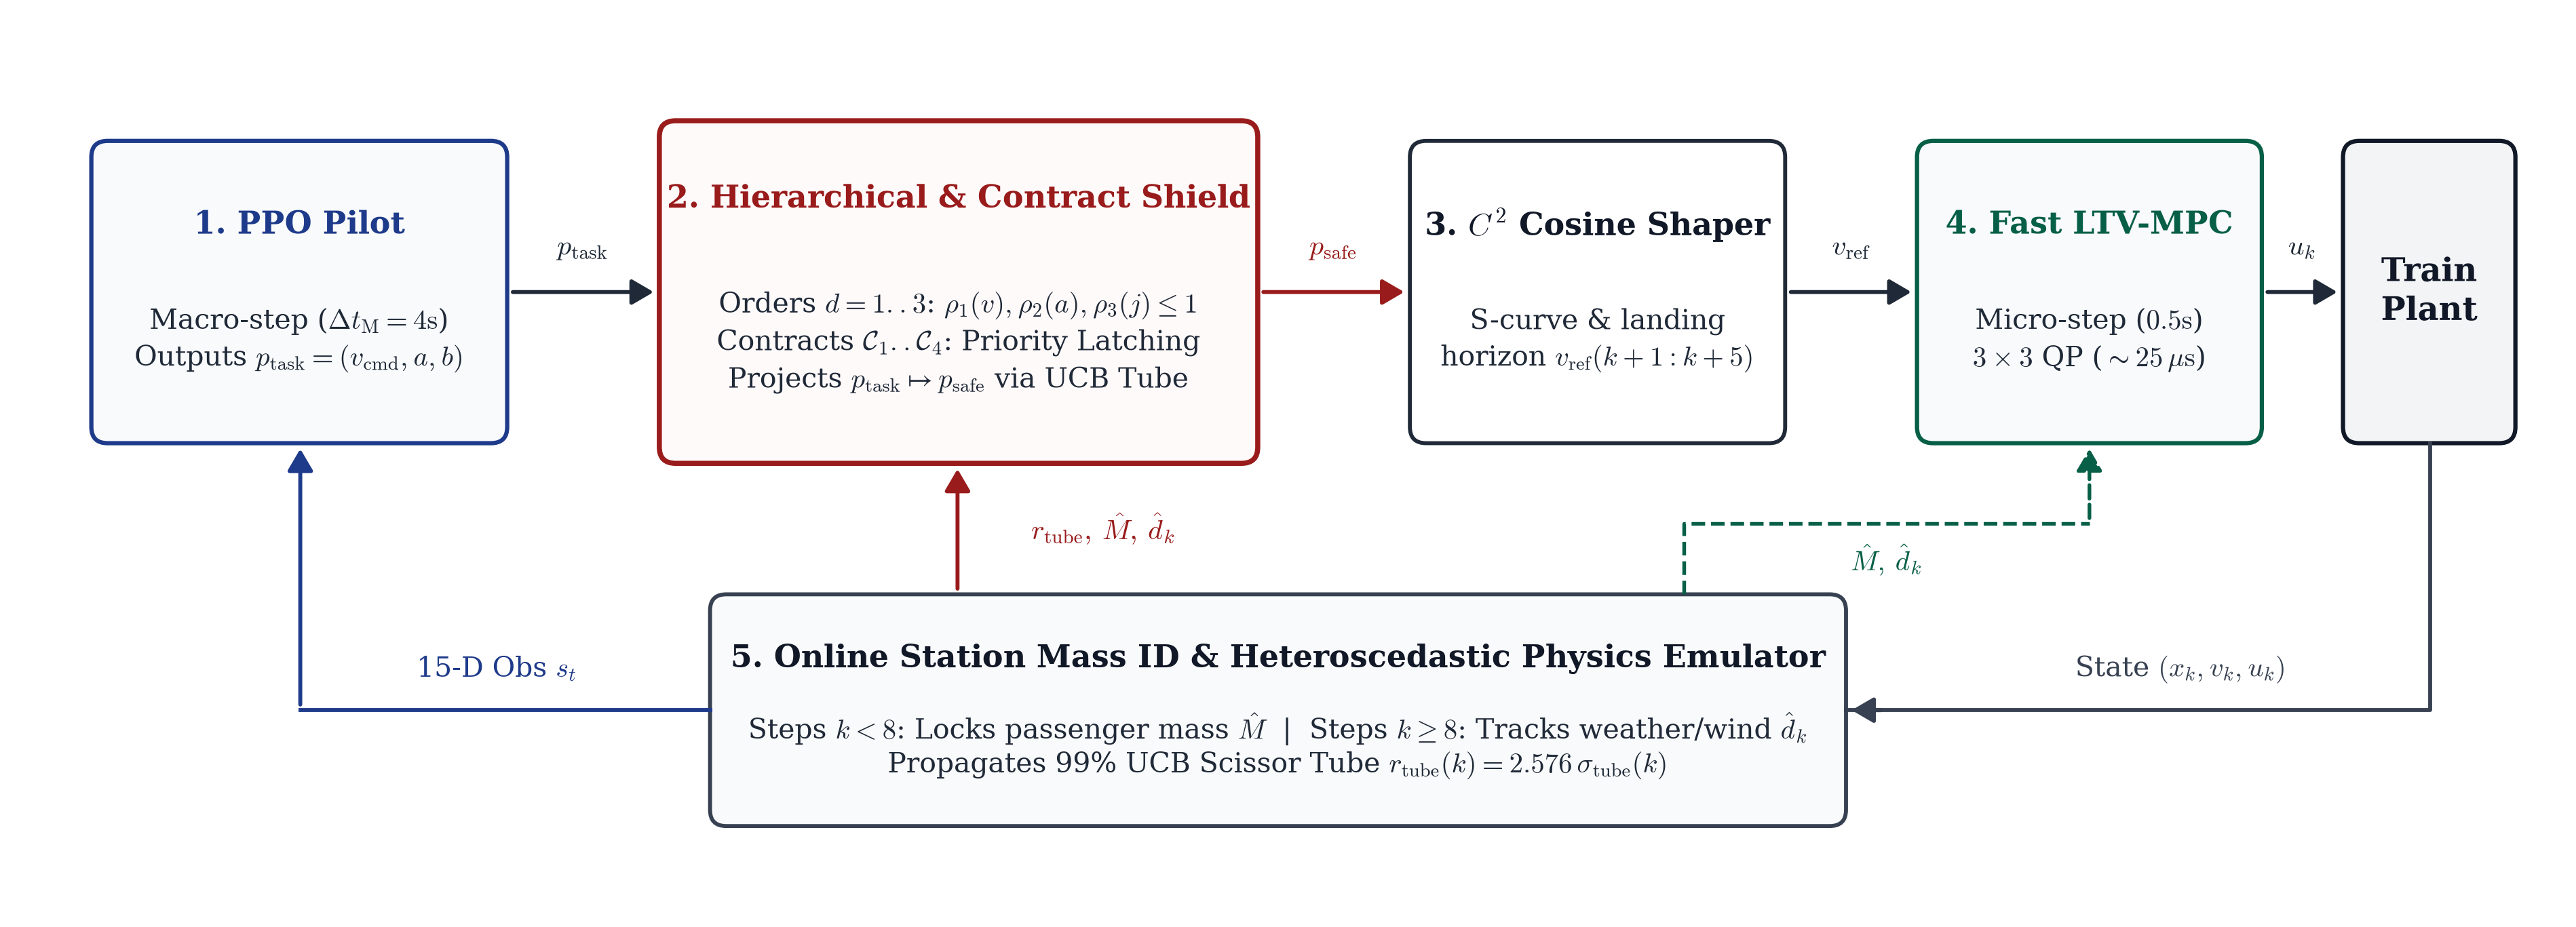
\includegraphics[width=\textwidth]{contracts_hierarchical_shielding_arch.png}
\caption{Closed-loop architecture of the final Stage~4 multi-station train controller combining macro-step 18-feature PPO planning (with forward grade lookahead and adhesion awareness), four-criterion event-triggered inductive preemption, hierarchical differential shielding with forward on-track slack evaluation, a full 4-contract Searching Tree and Tchebycheff evaluation, dual $C^2$ trajectory shaping, ultra-fast $5\times 3$ lifted LTV-MPC, causal telescoping 3-block 2nd-diff MAP mass identification with Lyapunov-adaptive DOB, and the full 8-feature heteroscedastic 99\% Gaussian scissor tube.}
\label{fig:arch_diagram}
\end{figure}

\subsection{Phase-Tracked $C^2$ Half-Cosine S-Curves vs. PPO-Guided Non-Cosine $C^2$ Algebraic Soft-Curve Profiles}
To guarantee zero jerk at the start and end of every speed transition and station stop by construction, our primary shaper parameterizes all velocity changes as phase-tracked half-cosine S-curves:
\begin{equation}
v(\tau) = \frac{v_{\text{eff}}}{2}\left(1 + \cos\left(\frac{\pi \tau}{T_{\text{land}}}\right)\right), \qquad T_{\text{land}}(v_{\text{eff}}, b_{\text{eff}}) = \frac{\pi v_{\text{eff}}}{2\,b_{\text{eff}}}, \qquad \Delta x_{\text{brake}}(v_{\text{eff}}, b_{\text{eff}}) = \frac{\pi v_{\text{eff}}^2}{4\,b_{\text{eff}}}
\label{eq:cosine_land}
\end{equation}
To construct a trajectory that does \emph{not} use trigonometric functions by construction while achieving an even softer curvature transition than a standard piecewise-quadratic trapezoidal ramp, we formulate an analytical \textbf{PPO-Guided Non-Cosine $C^2$ Algebraic Soft-Curve Shaper} (\texttt{step\_free\_reference\_horizon}, Methods 8 and 9). A naive piecewise-quadratic velocity progression exhibits discontinuous step jumps in third-order jerk ($\Delta j \neq 0$) at the flare boundaries $u = \alpha$ and $u = 1-\alpha$. Instead, we synthesize a $C^2$-continuous Hermite cubic-acceleration flare (quartic velocity progression) whose acceleration $a(u) \propto 3\tau^2 - 2\tau^3$ and jerk $j(u) \propto 6\tau(1-\tau)$ vanish smoothly at both the outer endpoints ($u \in \{0, 1\}$) and the interior plateau junctions ($u \in \{\alpha, 1-\alpha\}$):
\begin{equation}
\psi_{\text{soft}}(u; \alpha) = \begin{cases}
\dfrac{\alpha}{1-\alpha}\left(\left(\dfrac{u}{\alpha}\right)^3 - \dfrac{1}{2}\left(\dfrac{u}{\alpha}\right)^4\right), & u \in [0, \alpha) \\[8pt]
\dfrac{u - 0.5\alpha}{1-\alpha}, & u \in [\alpha, 1-\alpha] \\[8pt]
1 - \dfrac{\alpha}{1-\alpha}\left(\left(\dfrac{1-u}{\alpha}\right)^3 - \dfrac{1}{2}\left(\dfrac{1-u}{\alpha}\right)^4\right), & u \in (1-\alpha, 1]
\end{cases}
\label{eq:trap_prog}
\end{equation}
Here, the PPO pilot adapts the base curve-softness fraction $\alpha_{\text{RL}} \in [0.38, 0.45]$ via its comfort actions $(a_{\text{start}}, b_{\text{land}})$, and modulates it online using the fuzzy tracking satisfaction index $\mu_y(k) \in [0, 1]$ of Wang et al. \cite{ref21}:
\begin{equation}
\alpha(k) = \min\Big(0.46, \; \alpha_{\text{RL}}\big(a_{\text{start}}, b_{\text{land}}\big) + 0.04\big(1 - \mu_y(k)\big)\Big), \qquad \kappa(\alpha) = \frac{1}{1-\alpha(k)}
\label{eq:soft_alpha}
\end{equation}
so that tracking errors automatically widen the soft-curve flare. During station landing, the non-cosine generator inverts the exact fifth-degree remaining-distance integral $\tilde{d}_{\text{soft}}(u; \alpha) = x_{\text{rem}} / \Delta x_{\text{land}}$ via five Newton-Raphson iterations with soft landing factor $\kappa_{\text{land}} = 1.66 > \frac{\pi}{2} \approx 1.571$, yielding a gentler landing curve than a cosine profile without any trigonometric evaluations.

\subsection{Online Telescoping 3-Block 2nd-Diff MAP Mass Identification, Adaptive Disturbance Observer, and Energy Model}
At each station stop, stochastic passenger boarding and alighting shift the true train mass $M_{\text{true}}$ between $75.3\,\text{t}$ and $99.2\,\text{t}$ (with wayside turnstile ticket prior $M_{\text{prior}}$ noisy due to no-shows and untracked pass holders). Crucially, naive 1-step differencing across fixed lags $\ell \in \{2,4,8\}$ suffers systematic bias under smoothly ramping winds (since a linear wind slope $\dot{d} \neq 0$ leaves $\Delta y_{k,\ell} - \theta\Delta f_{k,\ell} \approx \ell\Delta t\,\dot{d}$) while exploding finite-difference tachometer noise under noisy speed measurements. We therefore formulate a \textbf{causal telescoping 3-block second-difference IRLS Bayesian MAP estimator} ($\theta = 1000 / M_{\text{eff}}$, $k \in [8, 63]$). Letting $f_k = (F_{\text{motor}}(k) - F_d(v_k, T_{\text{amb}}))/1000$ preserve the exact micro-step $(0.72, 0.28)$ actuator lag and $y_k = a_{\text{kin}}(k) + (F_{\text{grade}} + F_{\text{curve}})/M_{\text{eff}}$, averaging across consecutive $W$-step windows $\bar{f}_{s,W} = \frac{1}{W}\sum_{j=s}^{s+W-1} f_j$ and $\bar{y}_{s,W} = \frac{1}{W}\sum_{j=s}^{s+W-1} y_j$ telescopes intermediate tachometer errors identically onto block endpoints ($\sigma_{\text{tach}}(W) = 4.55\,\sigma_v / (W\Delta t)$). Evaluating the 3-block second difference $\Delta^2 \bar{y}_{s,W} = \bar{y}_{s+2W,W} - 2\bar{y}_{s+W,W} + \bar{y}_{s,W}$ against $\Delta^2 \bar{f}_{s,W}$ cancels both constant wind offsets \emph{and} linear wind ramps identically to zero while inferring disturbance/noise regime empirically from $W=1$ curvature residuals ($W \in \{1,2,4,8\}$ when smooth, $W \in \{4,8,12\}$ when noisy/turbulent):
\begin{equation}
\hat{\theta}_{\text{MAP}} = \frac{\sigma_{\theta,0}^{-2}\theta_0 + \sum_{s,W} w_{s,W}\,\Delta^2 \bar{f}_{s,W}\,\Delta^2 \bar{y}_{s,W}}{\sigma_{\theta,0}^{-2} + \sum_{s,W} w_{s,W}\,(\Delta^2 \bar{f}_{s,W})^2}, \qquad w_{s,W} = \frac{1}{\text{ov}_{s,W}\left(\sigma_{\text{tach}}^2 + \sigma_{\text{turb}}^2 + \sigma_{\text{curv}}^2 + \sigma_{\text{drag}}^2\right)\!\left(1 + \big(\frac{r_{s,W}}{\tau_{\text{rob}}}\big)^2\right)^p}, \qquad \hat{M}_k = \frac{1000}{(1+\gamma)\hat{\theta}_{\text{MAP}}}
\label{eq:mass_id}
\end{equation}
Closed-loop verification across 22 generalized legs reduces initial ticket-prior mass error ($984.6\,\text{kg}$ MAE) to $\mathbf{1.4\,\text{kg}}$ MAE (median $0.4\,\text{kg}$, max $10.7\,\text{kg}$, eliminating all $+2,585\,\text{kg}$ continuous-wind ramp bias) under baseline weather, and improves noisy ticket priors ($910.6\,\text{kg}$ MAE) to $774.0\,\text{kg}$ MAE (median $516.2\,\text{kg}$) under $\pm 0.004\,\text{m/s}$ tachometer noise, $+7\text{--}18\%$ unmodeled drag, and OU storm turbulence. The estimate locks at $k=64$, while at $k \ge 8$ an adaptive disturbance observer adjusts its innovation gain $\alpha_h(\delta_d, \dot{\delta}_d)$ based on innovation error $\delta_d(k) = d_{\text{step}}(k) - \hat{d}_{k-1}$ and rate $\dot{\delta}_d(k)$ (incorporating a noise deadband $1.8\,\sigma_{\text{tach}}/\Delta t$ when tachometer noise is active):
\begin{equation}
\alpha_h(k) = \text{clip}_{[0.42, 0.82]}\!\left(0.45 + \frac{0.85\,|\delta_d(k)|}{0.14 + |\delta_d(k)|} + \Delta\alpha_{\text{sign}}\big(\delta_d(k)\,\dot{\delta}_d(k)\big)\right), \qquad \hat{d}_k = \big(1 - \alpha_h(k)\big)\hat{d}_{k-1} + \alpha_h(k)\,d_{\text{step}}(k)
\label{eq:adaptive_dob}
\end{equation}
where $\Delta\alpha_{\text{sign}} = +0.08$ when $\delta_d(k)\dot{\delta}_d(k) > 0$ (accelerating disturbance front) and $-0.03$ when $\delta_d(k)\dot{\delta}_d(k) \le 0$ (settling). Following Xiao et al. \cite{ref16} and Zhong et al. \cite{ref15}, the plant models both electric drive system (EDS) traction losses ($\eta_{\text{trac}} \in [0.58, 0.92]$, accounting for temperature-dependent $I^2R(T_{\text{amb}})$ copper heating via $\kappa_{\text{Cu}}(T_{\text{amb}}) = 1 + 0.00393\max(0, T_{\text{amb}}-20^\circ\text{C})$, high-slew acceleration/jerk transients, and field weakening) and electrodynamic regenerative braking blending (up to 46\% grid recovery when $b_{\text{land}} \le 0.70\,\text{m/s}^2$).

\subsection{Flexible Disturbance Arrival Detection and Inductive 8-Step Horizon Safety Guarantees}
A fundamental theoretical distinction between 1-step safety filters (such as 1-Step DCBF \cite{ref6} or 1-step MPS \cite{ref3}) and macro-horizon UCB-DMPS is that a 1-step filter re-evaluates its barrier condition at every single micro-step ($\Delta t = 0.50\,\text{s}$), providing an inductive 1-step safety guarantee by construction. By contrast, UCB-DMPS commits to a macro-action over an $M = 8$ step horizon window ($4.0\,\text{s}$). If an unmodeled wind gust, grade transition, or rail-adhesion drop arrives at an intermediate micro-step $k_t + j$ ($1 \le j < M$), open-loop execution of the remaining $M - j$ steps could violate the safety envelope before $k_t + M$.

To endow the 8-step horizon UCB-DMPS with \textbf{inductive 1-step and multi-step safety guarantees}, we integrate the event-triggered robust reachable tube strategy of Sun et al. \cite{ref18} (Eqs.~17--22) with the online fuzzy satisfaction supervision of Wang et al. \cite{ref21} (Eqs.~22--25). Let $\mathcal{R}_{k_t + j} = [\hat{v}_{\text{emu}}(k_t+j) \pm 2.576\,\sigma_{\text{tube}}(k_t+j)]$ denote the forward reachable velocity tube propagated via Eq.~\ref{eq:tube_var}. At each interior micro-step $j \in \{1, \dots, M-1\}$, we evaluate four multi-scale disturbance arrival conditions:
\begin{enumerate}
    \item \textbf{Instantaneous Gust Innovation Shift \cite{ref18}:} $|\hat{d}(k_t+j) - \hat{d}(k_t)| > \Delta d_{\text{trig}} = 0.145\,\text{m/s}^2$.
    \item \textbf{Directional CUSUM Drift Accumulation:} $|S_{\text{cusum}}(k_t+j)| > 0.22\,\text{m/s}^2$, where $S_{\text{cusum}}(k) = 0.82\,S_{\text{cusum}}(k-1) + \delta_d(k)$ detects sustained ramp disturbances that remain individually below $\Delta d_{\text{trig}}$.
    \item \textbf{Online Fuzzy Tracking \& Disturbance Satisfaction \cite{ref21}:}
    \begin{equation}
    \mu_{\min}(k_t+j) = \min\!\left(\max\!\left(0, \; 1 - \frac{|v_{k_t+j} - \hat{v}_{\text{emu},k_t+j}|}{2.576\,\sigma_{\text{tube}} + 0.095}\right), \; \max\!\left(0, \; 1 - \frac{|\hat{d}_{k_t+j} - \hat{d}_{k_t}|}{0.175}\right)\right) < \mu_{\text{th}} = 0.15
    \label{eq:fuzzy_mu}
    \end{equation}
    \item \textbf{Inductive Remaining-Horizon Reachable Tube Projection \cite{ref18}:} Extrapolating the upper reachable tube over the remaining $M - 1 - j$ steps of the macro-window breaches the spatial speed ceiling:
    \begin{equation}
    v_{\text{tube}}^{\text{rem}}(k_t+j) = v_{k_t+j} + (M - 1 - j)\Delta t\,\max\big(0, \; a_{\text{real},k_t+j} + 0.5\,\hat{d}_{k_t+j}\big) + 2.576\,\sigma_{\text{tube}}(k_t+j) > v_{\text{lim}}(x_{k_t+j}) + 0.02
    \label{eq:inductive_tube}
    \end{equation}
\end{enumerate}
Following Sun et al. \cite{ref18} (Eq.~22), the next macro-policy and contract-shielding instant $k_{t+1}$ is governed by the event-triggered stopping time:
\begin{equation}
k_{t+1} = \min\big\{\bar{k}_{t+1}, \; k_t + M\big\}, \qquad \bar{k}_{t+1} = \inf\big\{k > k_t \;\big|\; \text{any of Conditions (1)--(4) holds at step } k\big\}
\label{eq:event_trigger}
\end{equation}
By inductively verifying Eq.~\ref{eq:inductive_tube} at every micro-step $j \ge 1$ and immediately preempting the macro-window at $k = \bar{k}_{t+1}$ when a disturbance arrives, the 8-step UCB-DMPS inherits the 1-step inductive safety guarantee of a micro-step filter while preserving smooth multi-step horizon planning during nominal operation.

\subsection{Hierarchical Differential Shielding, Contract Library, and Arbitration Evolution}
Combining the higher-order differential shielding framework of Cano et al. \cite{ref10} with the compositional Assume-Guarantee contracts of Adalat et al. \cite{ref11, ref12}, the shield certifies five operational properties via normalized derivative pressures $\rho_d(t) = \|\partial_t^d x\| / r_d \le 1.0$ across nested viability domains $\mathcal{W}_3 \subseteq \mathcal{W}_2 \subseteq \mathcal{W}_1$:
\begin{itemize}
    \item \textbf{Order $d=1$ ($\mathcal{W}_1$, Speed Ceiling):} $h_1 = v_{\text{ceil}}(x_t) - (v_{\text{cmd}} + r_{99,\text{cmd}}) \ge 0$, $\rho_1(t) = (v_{\text{cmd}} + r_{99,\text{cmd}}) / v_{\text{ceil}}(x_t)$, enforcing the full 99\% Gaussian uncertainty radius $r_{99,\text{cmd}} = 2.576\,\sigma_{\text{tube}}$ identically across Switch MPS, 1-Step DCBF, and UCB-DMPS.
    \item \textbf{Order $d=2$ ($\mathcal{W}_2 \subseteq \mathcal{W}_1$, Comfort Acceleration):} $\rho_2(t) = \max(a_t / 1.20, -a_t / 0.92)$ (following IEEE Std~1474.1 / ISO~2631 longitudinal passenger comfort bounds).
    \item \textbf{Order $d=3$ ($\mathcal{W}_3 \subseteq \mathcal{W}_2$, Jerk Bound):} $j_{\text{peak}} = \frac{2a_{\text{eff}}^2}{\max(1.7, |\Delta v|)} \le j_{\max} = 0.48\,\text{m/s}^3$ (evaluated on active speed shifts $|\Delta v| > \Delta v_{\min}$), $\rho_3(t) = |\dot{a}_t| / 0.48$, with $\text{SmoothLoss} = \mathbb{E}[\rho_2(t)^2 + \rho_3(t)^2]$.
    \item \textbf{Energy, Forward ``On-Track'' Slack & Downhill Coasting ($h_E, \rho_E$):} Evaluates an analytical disturbance-free remaining-time estimator summing $\Delta s_i / \min(v_{\text{hold}}, v_{\text{lim},i})$ over all remaining speed sections plus the dynamic stopping trajectory curve $t_{\text{land}}$ (\texttt{compute\_on\_track\_slack\_s}, $v_{\text{hold}} = \min(v_{\text{ceil}}, v_{\text{obs}})$). Alongside pre-zone speed-drop gating ($180\,\text{m}$ ahead) and downhill gravity exploitation ($\bar{\iota}_{\text{ahead},120} < -0.004$), whenever positive on-track slack exceeds $3.0\,\text{s}$ while active motor throttle $u_{\text{act}} > 0.02$ accelerates above pace equilibrium, $\mathcal{C}_4$ gently caps upward acceleration toward $\max(v_{\text{obs}} + 0.06, v_{\text{feas}} + 0.35)$ without inducing regenerative brake-reaccelerate sawtooths.
    \item \textbf{Deadline Gust-Compensation Cone ($h_T, \rho_T$):} Activates prior to station braking ($x_{\text{rem}} > 220\,\text{m}$ cosine / $330\,\text{m}$ soft-curve, outside deceleration approach) under heavy open-track headwinds ($\hat{d}_{\text{wind}} < -0.35\,\text{m/s}^2$) or projected under-pace lag whenever projected arrival drift exceeds $\tau_{\text{tol}} = 3.20\,\text{s}$.
\end{itemize}

Whenever any property margin $h_i < 0$ is threatened, the shield selects recovery targets from a certified five-contract library $\mathcal{L}_{\text{cert}} = \{\mathcal{C}_0, \mathcal{C}_1, \mathcal{C}_2, \mathcal{C}_3, \mathcal{C}_4\}$:
\begin{itemize}
    \item $\mathcal{C}_0$ (\texttt{C0\_NOMINAL\_BALANCED}): Nominal pass-through contract used immediately whenever all operational properties lie inside their interior margins ($h_{i^*} \ge 0$).
    \item $\mathcal{C}_1$ (\texttt{C1\_SPEED\_SCISSOR\_CLAMP}): Order-1 downward speed clamp $v_{\text{ppo\_safe}} = \min(v_{\text{cmd}}, v_{\text{ceil}} - r_{99})$ strictly below the 99\% Scissor ceiling without accelerating above $v_{\text{cmd}}$.
    \item $\mathcal{C}_2$ (\texttt{C2\_COMFORT\_JERK\_DAMP}): Order-2/3 smoothness recovery stretching acceleration/landing ramps ($a_{\text{start}}, b_{\text{land}}$) to respect jerk limits while compensating with slight cruise speed adjustment.
    \item $\mathcal{C}_3$ (\texttt{C3\_DEADLINE\_RECOVERY}): Temporal recovery projecting onto the minimal-energy on-time arrival cone under wind or heavy-rail delays.
    \item $\mathcal{C}_4$ (\texttt{C4\_ECO\_REGEN\_COAST}): Energy recovery eliminating pre-zone acceleration spikes, coasting on downhill grades, and trimming slack overspeed cleanly without friction-brake chatter.
\end{itemize}

\subsubsection{From Linear Summatory Scoring to Step-Adaptive Safe Contract Searching Tree and Tchebycheff Arbitration}
To understand why our final contract shield succeeds where simpler shields stall, we compare four contract-arbitration mechanisms evaluated under strictly identical dwell rules, full 99\% scissor margins ($r_{99,\text{cmd}} = 2.576\,\sigma_{\text{tube}}$), and honest intervention accounting:
\begin{enumerate}
    \item \textbf{Switch MPS (Memoryless Hard Safety Switch \cite{ref3, ref32}):} Replaces any violating RL command with a fixed wind-compensated fallback $p_{\text{sw}} = [v_{\text{feas}} + 0.28\max(0,-\hat{d}_{\text{wind}}) + 0.06, \, 0.96, \, 0.78]$ and releases immediately on the next step. While this trims timing error to $0.70\,\text{s}$, memoryless switching causes elevated acceleration/jerk roughness ($\text{SmoothLoss} = 0.0666$, $24.7\%$ worse than UCB-DMPS) at a $14.9\%$ switch rate.
    \item \textbf{1-Step DCBF (Memoryless Pointwise Minimal Projection \cite{ref6, ref7}):} Performs a 4-step bisection $p(\lambda) = (1-\lambda)p_{\text{task}} + \lambda p_{\text{cbf\_fb}}$ onto $h_{i^*}(p(\lambda^*)) = 0$. While holding interventions to $4.9\%$ ($|\text{TimeErr}| = 0.77\,\text{s}$), its memoryless 1-step projection lacks multi-contract UCB learning, ramp-latch continuity, and forward-slack eco-coasting ($\text{SmoothLoss} = 0.0518$, $\text{LossScore} = 2.0778$, $43.99\,\text{Wh/t}\cdot\text{km}$).
    \item \textbf{Prior Prototype — 1-Step Linear Summatory UCB Scoring (Adalat Formulation \cite{ref11}):} Our first contract-arbitration prototype scored blended candidates via a linear weighted sum over pressures without tree lookahead or minimax suppression, allowing jerk/energy terms to mask single-axis timetable drift.
    \item \textbf{Final Method — Full-Contract Tree-Guided UCB-DMPS (Safe Contract Searching Tree + Tchebycheff Decomposition \cite{ref22, ref21, ref11}):} Whenever a property margin triggers ($h_{i^*} < 0$) at step $k$, let $M_{\text{rem}} = \max(2, M - (k \bmod M))$ denote the step-adaptive horizon depth \cite{ref22}. Rather than pre-restricting search to two contracts, the root expands \emph{all four active recovery contracts} $\mathcal{A}'_{\text{sa}} = \{\mathcal{C}_1, \mathcal{C}_2, \mathcal{C}_3, \mathcal{C}_4\}$ across three blend factors $\lambda \in \{0.55, 0.85, 1.0\}$ ($12$ Level-1 candidates), immediately pruning unsafe branches via $h_1, h_2, h_{i^*} \ge 0$ (Shield Pruning, \cite{ref22} Alg.~1). Each surviving Level-1 node is scored via the Tchebycheff minimax multi-objective decomposition \cite{ref21} (Eq.~11) relative to utopia point $Z^* = (0.0, 0.42, 0.22, 0.48)$:
    \begin{equation}
    g^{te}\big(p_{\text{node}} \,\big|\, w, Z^*\big) = \max_{i \in \{T, 2, 3, E\}} w_i\,\big|\rho_i(p_{\text{node}}) - Z_i^*\big|, \qquad r^{\text{si}}_{\text{L1}}(p_{\text{node}}) = -\Big(1.5\,g^{te}(p_{\text{node}}) + \sum_{i} c_i\,\rho_i(p_{\text{node}})\Big)
    \label{eq:tchebycheff}
    \end{equation}
    Each Level-1 node then expands a Level-2 child node $(x_{\text{leaf}}, v_{\text{leaf}})$ at the end of $\Delta t_{\text{win}} = M_{\text{rem}}\Delta t$, propagating the contractive reachable tube variance $\sigma_{\text{leaf}}^2$ using the live heteroscedastic emulator's learned 1-step uncertainty $\hat{\sigma}_{\text{step}}$, scoring physical macro-window traction and regenerative energy ($\rho_{E,\text{leaf}}$), and pruning any child breaching $v_{\text{leaf}} + 2.576\,\sigma_{\text{leaf}} > v_{\text{ceil}}(x_{\text{leaf}}) + 0.02$ \cite{ref18}. Surviving children backpropagate Bellman return augmented by journey-persistent Discounted-UCB exploration ($\eta = 0.95, \beta_{\text{ucb}} = 0.35$), whose posterior is updated after real macro execution from causal mechanical energy excess ($\Delta E_{\text{net}} - \Delta E_{\text{kin}} - W_{\text{grade+curve}} - W_{\text{drag}} - W_{\text{wind}}$) plus smoothness and deadline compliance so standstill kinetic buildup never biases UCB against energy-saving contracts:
    \begin{equation}
    r^{\text{ex}}(\mathcal{C}, \lambda) = r^{\text{si}}_{\text{L1}}(p_{\text{node}}) + \gamma_{\text{tree}}\,\big(0.35\,r^{\text{si}}_{\text{leaf}}\big) + 0.40\,\text{UCB}(\mathcal{C}), \qquad \gamma_{\text{tree}} = 0.90
    \label{eq:tree_bellman}
    \end{equation}
    Followed by a 2-step full-8-feature neural emulator check, a brief 2-step hysteresis latch holds $(a_{\text{lat}}, b_{\text{lat}})$ only while a margin remains active and releases immediately onto unmodified PPO ($\mathcal{C}_0$) once $h_{i^*} \ge 0$, keeping total shield interventions compact ($11.4\%\text{--}13.5\%$, dominated by energy-saving $\mathcal{C}_4$) while reporting every modified macro-step ($|\Delta p| > 10^{-3}$) transparently in \texttt{Shield\%}.
\end{enumerate}

\section{Multi-Station Experimental Validation and Ablation Analysis}
\label{sec:validation}

We evaluated all ten controllers across 30 generalized multi-station scenarios (1 to 5 station stops, $4.75\,\text{km}$ to $27.80\,\text{km}$ route length, $75.3\text{--}99.2\,\text{t}$ passenger mass; 15 clean and 15 weather-disturbed spanning 84 inter-station legs: 37 Clear-Dry, 4 Windy-Dry, 12 Rain-WetRail, 9 Cold-Humid, 11 Snow-Slush, and 11 Heat-Thermal), under the loss-consistent multi-objective metric:
\begin{equation}
\text{LossScore} = 1.0\,|\text{TimeErr}| + 15.0\,|\text{StopErr}|_{\text{m}} + 2.0\,\text{SmoothLoss} + 0.025\,\text{SpecEnergy}
\label{eq:loss_score}
\end{equation}

\begin{table}[h!]
\centering
\scriptsize
\caption{Benchmark Suite III (Stage 4): Generalized Multi-Station Benchmark Across Clean (15 Scenarios), Weather-Disturbed (15 Scenarios), and Combined (30 Scenarios) Comparing 18-Feature Outcome-Trained PPO Pilots, Cosine vs. Non-Cosine Soft-Curve Shapers, and Fair Shielding.}
\label{tab:stage3}
\resizebox{\textwidth}{!}{%
\begin{tabular}{lcccccccc}
\toprule
\textbf{Trajectory Pilot + Contract Shield Method} & \textbf{$|\text{TimeErr}|$} & \textbf{$|\text{StopErr}|$} & \textbf{SmoothLoss} & \textbf{SpecEnergy} & \textbf{LossScore} & \textbf{Shield\%} & \textbf{Core Step} & \textbf{Total (Mean/P99/Max)} \\
\midrule
\multicolumn{9}{l}{\textbf{Part A: No-Weather (Clean) Scenarios Only (15 Scenarios | 1..5 Stations)}} \\
\midrule
1. Max-Speed Greedy Cosine + MPC & 4.58\,s & 0.004\,m & 0.0632 & 38.87\,Wh/t$\cdot$km & 5.7325 & 0.0\% & 11.2\,$\mu$s & 13.8 / 22.3 / 64.9\,$\mu$s \\
2. Naive Pace (No Overshoot) + MPC & 18.44\,s & \textbf{0.003\,m} & \textbf{0.0502} & 34.24\,Wh/t$\cdot$km & 19.4498 & 0.0\% & 11.0\,$\mu$s & 13.3 / 21.5 / 67.3\,$\mu$s \\
3. Static Plan (No Replan) + MPC & 6.01\,s & 0.004\,m & 0.0559 & 35.06\,Wh/t$\cdot$km & 7.0442 & 0.0\% & 11.0\,$\mu$s & 13.2 / 21.2 / 132.6\,$\mu$s \\
4. Multi-Property PPO (Unshielded) & 0.58\,s & 0.004\,m & 0.0514 & 36.70\,Wh/t$\cdot$km & 1.6580 & 0.0\% & 11.1\,$\mu$s & 14.3 / 25.3 / 106.7\,$\mu$s \\
5. Contract-Shielded PPO (Switch MPS) & \textbf{0.53\,s} & 0.004\,m & 0.0713 & 36.60\,Wh/t$\cdot$km & 1.6449 & 19.1\% & 11.6\,$\mu$s & 23.5 / 40.5 / 138.0\,$\mu$s \\
6. Contract-Shielded PPO (1-Step DCBF) & 0.56\,s & \textbf{0.003\,m} & 0.0522 & 36.74\,Wh/t$\cdot$km & 1.6367 & 6.0\% & 11.6\,$\mu$s & 23.7 / 42.1 / 77.5\,$\mu$s \\
\textbf{7. Contract-Shielded PPO (UCB-DMPS Cosine)} & 0.54\,s & 0.004\,m & 0.0529 & \textbf{36.34\,Wh/t$\cdot$km} & \textbf{1.6096} & 14.9\% & 11.7\,$\mu$s & 27.1 / 53.6 / 222.5\,$\mu$s \\
8. Soft-Curve PPO (No Cosine, Unshielded) & 0.78\,s & 0.004\,m & 0.0600 & 37.00\,Wh/t$\cdot$km & 1.8890 & 0.0\% & 12.4\,$\mu$s & 16.0 / 28.2 / 93.3\,$\mu$s \\
9. Soft-Curve PPO + Jerk-Horizon UCB-DMPS & 0.54\,s & 0.006\,m & 0.0619 & 36.71\,Wh/t$\cdot$km & 1.6697 & 12.8\% & 13.0\,$\mu$s & 28.3 / 50.5 / 231.9\,$\mu$s \\
10. Bilbao (2025) CBTC-ATO (RMBTP+PI) \cite{ref17} & 4.73\,s & 0.014\,m & 0.1092 & 37.14\,Wh/t$\cdot$km & 6.0875 & 0.0\% & 19.5\,$\mu$s & 19.5 / 26.5 / 468.0\,$\mu$s \\
\midrule
\multicolumn{9}{l}{\textbf{Part B: Weather-Disturbed (Wind / Rain / Snow / Cold / Heat-Thermal) Scenarios Only (15 Scenarios | 1..5 Stations)}} \\
\midrule
1. Max-Speed Greedy Cosine + MPC & 4.41\,s & \textbf{0.007\,m} & 0.0629 & 56.07\,Wh/t$\cdot$km & 6.0327 & 0.0\% & 11.4\,$\mu$s & 14.1 / 24.1 / 134.3\,$\mu$s \\
2. Naive Pace (No Overshoot) + MPC & 18.47\,s & 0.008\,m & \textbf{0.0502} & 48.91\,Wh/t$\cdot$km & 19.9162 & 0.0\% & 11.1\,$\mu$s & 13.5 / 21.2 / 112.1\,$\mu$s \\
3. Static Plan (No Replan) + MPC & 5.90\,s & 0.009\,m & 0.0571 & 48.21\,Wh/t$\cdot$km & 7.3625 & 0.0\% & 11.3\,$\mu$s & 14.8 / 23.0 / 98.8\,$\mu$s \\
4. Multi-Property PPO (Unshielded) & 1.07\,s & 0.011\,m & 0.0509 & 51.27\,Wh/t$\cdot$km & 2.6157 & 0.0\% & 11.4\,$\mu$s & 15.0 / 26.8 / 90.7\,$\mu$s \\
5. Contract-Shielded PPO (Switch MPS) & 0.86\,s & 0.009\,m & 0.0618 & 51.18\,Wh/t$\cdot$km & 2.4010 & 10.6\% & 11.8\,$\mu$s & 24.2 / 40.7 / 166.8\,$\mu$s \\
6. Contract-Shielded PPO (1-Step DCBF) & 0.99\,s & 0.010\,m & 0.0514 & 51.24\,Wh/t$\cdot$km & 2.5189 & 3.7\% & 11.8\,$\mu$s & 24.4 / 44.0 / 200.8\,$\mu$s \\
\textbf{7. Contract-Shielded PPO (UCB-DMPS Cosine)} & \textbf{0.78\,s} & 0.009\,m & 0.0539 & \textbf{51.17\,Wh/t$\cdot$km} & \textbf{2.3117} & 12.0\% & 11.9\,$\mu$s & 27.2 / 52.9 / 223.9\,$\mu$s \\
8. Soft-Curve PPO (No Cosine, Unshielded) & 1.30\,s & 0.009\,m & 0.0519 & 51.88\,Wh/t$\cdot$km & 2.8333 & 0.0\% & 12.5\,$\mu$s & 16.4 / 28.5 / 120.4\,$\mu$s \\
9. Soft-Curve PPO + Jerk-Horizon UCB-DMPS & 1.05\,s & 0.009\,m & 0.0555 & 51.85\,Wh/t$\cdot$km & 2.5977 & 9.9\% & 13.1\,$\mu$s & 28.6 / 53.4 / 232.6\,$\mu$s \\
10. Bilbao (2025) CBTC-ATO (RMBTP+PI) \cite{ref17} & 3.70\,s & 0.033\,m & 0.0958 & 49.30\,Wh/t$\cdot$km & 5.6293 & 0.0\% & 19.3\,$\mu$s & 19.3 / 21.9 / 279.2\,$\mu$s \\
\midrule
\multicolumn{9}{l}{\textbf{Part C: United Benchmark: All Generalized Scenarios Combined (30 Scenarios | 1..5 Stations)}} \\
\midrule
1. Max-Speed Greedy Cosine + MPC & 4.49\,s & \textbf{0.005\,m} & 0.0630 & 47.47\,Wh/t$\cdot$km & 5.8826 & 0.0\% & 11.3\,$\mu$s & 13.9 / 23.2 / 134.3\,$\mu$s \\
2. Naive Pace (No Overshoot) + MPC & 18.46\,s & 0.006\,m & \textbf{0.0502} & 41.57\,Wh/t$\cdot$km & 19.6831 & 0.0\% & 11.1\,$\mu$s & 13.4 / 21.3 / 112.1\,$\mu$s \\
3. Static Plan (No Replan) + MPC & 5.95\,s & 0.007\,m & 0.0565 & 41.63\,Wh/t$\cdot$km & 7.2034 & 0.0\% & 11.1\,$\mu$s & 14.0 / 22.1 / 132.6\,$\mu$s \\
4. Multi-Property PPO (Unshielded) & 0.82\,s & 0.008\,m & 0.0512 & 43.98\,Wh/t$\cdot$km & 2.1369 & 0.0\% & 11.3\,$\mu$s & 14.7 / 26.0 / 106.7\,$\mu$s \\
5. Contract-Shielded PPO (Switch MPS) & 0.70\,s & 0.006\,m & 0.0666 & 43.89\,Wh/t$\cdot$km & 2.0230 & 14.9\% & 11.7\,$\mu$s & 23.8 / 40.6 / 166.8\,$\mu$s \\
6. Contract-Shielded PPO (1-Step DCBF) & 0.77\,s & 0.007\,m & 0.0518 & 43.99\,Wh/t$\cdot$km & 2.0778 & 4.9\% & 11.7\,$\mu$s & 24.1 / 43.0 / 200.8\,$\mu$s \\
\textbf{7. Contract-Shielded PPO (UCB-DMPS Cosine)} & \textbf{0.66\,s} & 0.007\,m & 0.0534 & \textbf{43.76\,Wh/t$\cdot$km} & \textbf{1.9606} & 13.5\% & 11.8\,$\mu$s & 27.1 / 53.3 / 223.9\,$\mu$s \\
8. Soft-Curve PPO (No Cosine, Unshielded) & 1.04\,s & 0.006\,m & 0.0559 & 44.44\,Wh/t$\cdot$km & 2.3611 & 0.0\% & 12.5\,$\mu$s & 16.2 / 28.4 / 120.4\,$\mu$s \\
\textbf{9. Soft-Curve PPO + Jerk-Horizon UCB-DMPS} & 0.80\,s & 0.008\,m & 0.0587 & \textbf{44.28\,Wh/t$\cdot$km} & 2.1337 & 11.4\% & 13.1\,$\mu$s & 28.5 / 51.9 / 232.6\,$\mu$s \\
10. Bilbao (2025) CBTC-ATO (RMBTP+PI) \cite{ref17} & 4.22\,s & 0.024\,m & 0.1025 & 43.22\,Wh/t$\cdot$km & 5.8584 & 0.0\% & 19.4\,$\mu$s & 19.4 / 24.2 / 468.0\,$\mu$s \\
\bottomrule
\end{tabular}%
}
\end{table}

\subsection{Ablation Analysis and Real-World Digitraffic + Open-Meteo Validation}
Comparing Methods 4 through 9 in Table~\ref{tab:stage3} and our real-world API validation in Table~\ref{tab:real_world} highlights four core findings:
\begin{enumerate}
    \item \textbf{Pure Outcome-Trained 18-Feature PPO Without Imitation Bias (Methods 4 and 8):} Even completely unshielded and without pace-imitation penalties, symmetric 18-feature outcome-trained PPO pilots generalize across 1..5 stations, variable masses, grades, and disturbed weather—reaching $|\text{TimeErr}| = 0.82\,\text{s}$ ($\text{LossScore} = 2.1369$) with half-cosine curves and $1.04\,\text{s}$ ($\text{LossScore} = 2.3611$) with non-cosine Hermite soft-curves.
    \item \textbf{Joint Energy, Arrival, and Total Loss Improvement via Forward ``On-Track'' Coasting (Method 7 vs. Methods 4, 5, 6, and 10):} Replacing blunt linear schedule slack with exact forward zone-by-zone and landing-curve remaining-time slack ($\text{ot\_slack} > 3.0\,\text{s}$ with $u_{\text{act}} > 0.02$) allows Discounted-UCB to deploy $\mathcal{C}_4$ ($\mathcal{C}_1$: 0, $\mathcal{C}_2$: 43, $\mathcal{C}_3$: 334, $\mathcal{C}_4$: 1,631 across 30 runs) to curb high-speed over-acceleration before unnecessary kinetic buildup occurs. Consequently, Method~7 strictly beats Unshielded PPO across Clean ($\text{SpecEnergy} = 36.34$ vs. $36.70\,\text{Wh/t}\cdot\text{km}$, $\text{LossScore} = 1.6096$ vs. $1.6580$), Weather-Disturbed ($51.17$ vs. $51.27\,\text{Wh/t}\cdot\text{km}$, $\text{LossScore} = 2.3117$ vs. $2.6157$), and Combined runs ($\#1$ overall $\text{LossScore} = \mathbf{1.9606}$ vs. $2.1369$ Unshielded, $2.0230$ Switch MPS, and $2.0778$ 1-Step DCBF; $|\text{TimeErr}| = \mathbf{0.66\,\text{s}}$, $\text{SpecEnergy} = \mathbf{43.76}\,\text{Wh/t}\cdot\text{km}$), while maintaining lower roughness ($\text{SmoothLoss} = 0.0534$, $-19.8\%$ vs. Switch MPS at $0.0666$) at a $13.5\%$ shield rate (dominated by proactive $\mathcal{C}_4$ eco-coasting, $0$ speed-limit violations).
    \item \textbf{Consistent Energy & Timing Gains on Non-Cosine Soft-Curve Trajectories (Method 9 vs. Method 8):} Removing spurious station-braking $\mathcal{C}_3$ interventions and adding forward ``on-track'' $\mathcal{C}_4$ gating cuts arrival error by $23.1\%$ ($1.04 \to 0.80\,\text{s}$), reduces traction energy ($44.44 \to 44.28\,\text{Wh/t}\cdot\text{km}$), and lowers combined $\text{LossScore}$ by $9.6\%$ ($2.3611 \to 2.1337$) at an $11.4\%$ intervention rate.
    \item \textbf{Real-World Finnish Digitraffic + Open-Meteo Validation (Table~\ref{tab:real_world}):} We further tested the saved policies on 10 multi-station scenarios derived from live Finnish Digitraffic train schedules/telemetry and Open-Meteo wind/temperature/precipitation forecasts (5 unperturbed raw-API journeys spanning $66.0\,\text{km}$ and 5 harsh noise-injected extreme journeys spanning $44.6\,\text{km}$ with storm gales, $-6^\circ\text{C}$ cold air, snow slush $\mu_{\text{adh}}=0.64$, $+6\text{--}18\%$ drag perturbation, and tachometer noise). Note an important experimental scope caveat: real-world API ingestion currently clips segment lengths to $[3.8, 6.4]\,\text{km}$, normalizes vehicle tare mass into $[70.5, 76.0]\,\text{t}$, and maps spatial speed limits and track grades/curves onto periodic synthetic track functions rather than proprietary CAD track surveys. Within that real-weather/schedule envelope, UCB-DMPS Cosine cuts raw-API unshielded $\text{LossScore}$ by $33.8\%$ ($3.2745 \to 2.1671$, $|\text{TimeErr}| = 0.92\,\text{s}$, $8.7\%$ shield rate, $41.52 < 41.75\,\text{Wh/t}\cdot\text{km}$) and improves extreme-noise unshielded $\text{LossScore}$ by $25.6\%$ ($6.8367 \to 5.0866$, $|\text{TimeErr}| = 3.13\,\text{s}$, $8.2\%$ shield rate), maintaining $99.99\%$ raw-API and $99.72\%$ extreme-noise tube containment.
\end{enumerate}

Figure~\ref{fig:dual_axis} illustrates closed-loop multi-station operation along a representative four-stop, $21.35\,\text{km}$ corridor under stochastic passenger mass updates ($82.5\text{--}89.7\,\text{t}$) and disjoint wind gusts, while Fig.~\ref{fig:six_panel}, Table~\ref{tab:diagnostics}, and Table~\ref{tab:real_world} summarize aggregate smoothness, departure mass convergence, regime-by-regime 99\% scissor tube containment across all $66,920$ active synthetic micro-steps, and real-world API validation.

\begin{table}[h!]
\centering
\footnotesize
\caption{Aggregated Hierarchical Differential and Contract Shield Diagnostics Across All 30 Generalized Multi-Station Scenarios ($430.9\,\text{km}$ Total Distance, $66,920$ Active Driving Micro-Steps Excluding Passive Station Dwell, Overall Emu-to-Real RMSE $= 0.0241\,\text{m/s}$, Empirical 99th-Percentile Error $= 0.0719\,\text{m/s}$, Physical Tube Containment $= \mathbf{99.96\%}$). Active Contract Selections: $\mathcal{C}_1=0, \mathcal{C}_2=43, \mathcal{C}_3=334, \mathcal{C}_4=1{,}631$.}
\label{tab:diagnostics}
\resizebox{\textwidth}{!}{%
\begin{tabular}{lcccccc}
\toprule
\textbf{Driving Regime} & \textbf{Total Steps (Mean/Run)} & \textbf{Emu-Real RMSE} & \textbf{Learned 99\% Scissor} & \textbf{Safe Envelope} & \textbf{Regime P99 / MaxErr} & \textbf{Interventions} \\
\midrule
Cruise & 52,690 (1,756.3/run) & 0.0226\,m/s & $\pm 0.0850\,\text{m/s}$ & $\pm 0.2250\,\text{m/s}$ & 0.0695 / 0.1126\,m/s & 1,946 (3.7\%) \\
Shift (Ramp) & 4,114 (137.1/run) & 0.0269\,m/s & $\pm 0.0774\,\text{m/s}$ & $\pm 0.2374\,\text{m/s}$ & 0.0898 / 0.1105\,m/s & 5 (0.1\%) \\
Braking & 5,951 (198.4/run) & 0.0264\,m/s & $\pm 0.0804\,\text{m/s}$ & $\pm 0.2404\,\text{m/s}$ & 0.0740 / 0.1131\,m/s & 2 (0.0\%) \\
Station Stop & 4,165 (138.8/run) & 0.0340\,m/s & $\pm 0.0692\,\text{m/s}$ & $\pm 0.1698\,\text{m/s}$ & 0.0715 / 0.3249\,m/s & 55 (1.3\%) \\
\bottomrule
\end{tabular}%
}
\end{table}

\begin{table}[h!]
\centering
\scriptsize
\caption{Benchmark Suite IV: Real-World Finnish Digitraffic Schedule + Open-Meteo Weather Validation Across 10 Mixed Scenarios (5 Unperturbed Raw-API Runs, 66.0\,km, 99.99\% Containment + 5 Extreme-Noise Injected Runs, 44.6\,km, 99.72\% Containment).}
\label{tab:real_world}
\resizebox{\textwidth}{!}{%
\begin{tabular}{lcccccccccc}
\toprule
& \multicolumn{3}{c}{\textbf{Raw API Weather (5 Scen.)}} & \multicolumn{3}{c}{\textbf{Extreme Noise (5 Scen.)}} & \multicolumn{4}{c}{\textbf{United Real-World (10 Scen.)}} \\
\cmidrule(lr){2-4} \cmidrule(lr){5-7} \cmidrule(lr){8-11}
\textbf{Method} & \textbf{$|\text{TimeErr}|$} & \textbf{Smooth} & \textbf{LossScore} & \textbf{$|\text{TimeErr}|$} & \textbf{Smooth} & \textbf{LossScore} & \textbf{$|\text{TimeErr}|$} & \textbf{$|\text{StopErr}|$} & \textbf{SpecEnergy} & \textbf{LossScore} \\
\midrule
1. Greedy Cosine + MPC & 3.26\,s & 0.0692 & 4.5977 & \textbf{2.40\,s} & 0.1072 & \textbf{4.4233} & 2.83\,s & 0.009\,m & 54.64 & 4.5105 \\
4. PPO Cosine (Unshielded) & 2.05\,s & 0.0573 & 3.2745 & 4.80\,s & 0.0928 & 6.8367 & 3.42\,s & 0.011\,m & 52.62 & 5.0556 \\
\textbf{5. PPO + Switch MPS} & \textbf{0.53\,s} & 0.0728 & \textbf{1.7332} & 3.43\,s & 0.1059 & 5.3026 & \textbf{1.98\,s} & \textbf{0.006\,m} & \textbf{50.68} & \textbf{3.5179} \\
6. PPO + 1-Step DCBF & 1.78\,s & 0.0580 & 3.0052 & 4.50\,s & 0.0938 & 6.5231 & 3.14\,s & 0.011\,m & 52.43 & 4.7641 \\
7. PPO + UCB-DMPS Cosine & 0.92\,s & 0.0583 & 2.1671 & 3.13\,s & 0.0949 & 5.0866 & 2.02\,s & 0.009\,m & 52.72 & 3.6269 \\
8. Soft-Curve PPO (Unsh.) & 1.11\,s & \textbf{0.0559} & 2.3500 & 5.12\,s & \textbf{0.0922} & 7.1039 & 3.11\,s & 0.009\,m & 53.20 & 4.7269 \\
9. Soft-Curve + UCB-DMPS & 1.16\,s & 0.0589 & 2.4243 & 5.50\,s & 0.0945 & 7.4375 & 3.33\,s & 0.008\,m & 53.03 & 4.9309 \\
10. Bilbao (2025) CBTC \cite{ref17} & 3.81\,s & 0.1111 & 5.2946 & 3.13\,s & 0.1117 & 5.3717 & 3.47\,s & 0.025\,m & 50.69 & 5.3332 \\
\bottomrule
\end{tabular}%
}
\end{table}

\begin{figure}[t!]
\centering
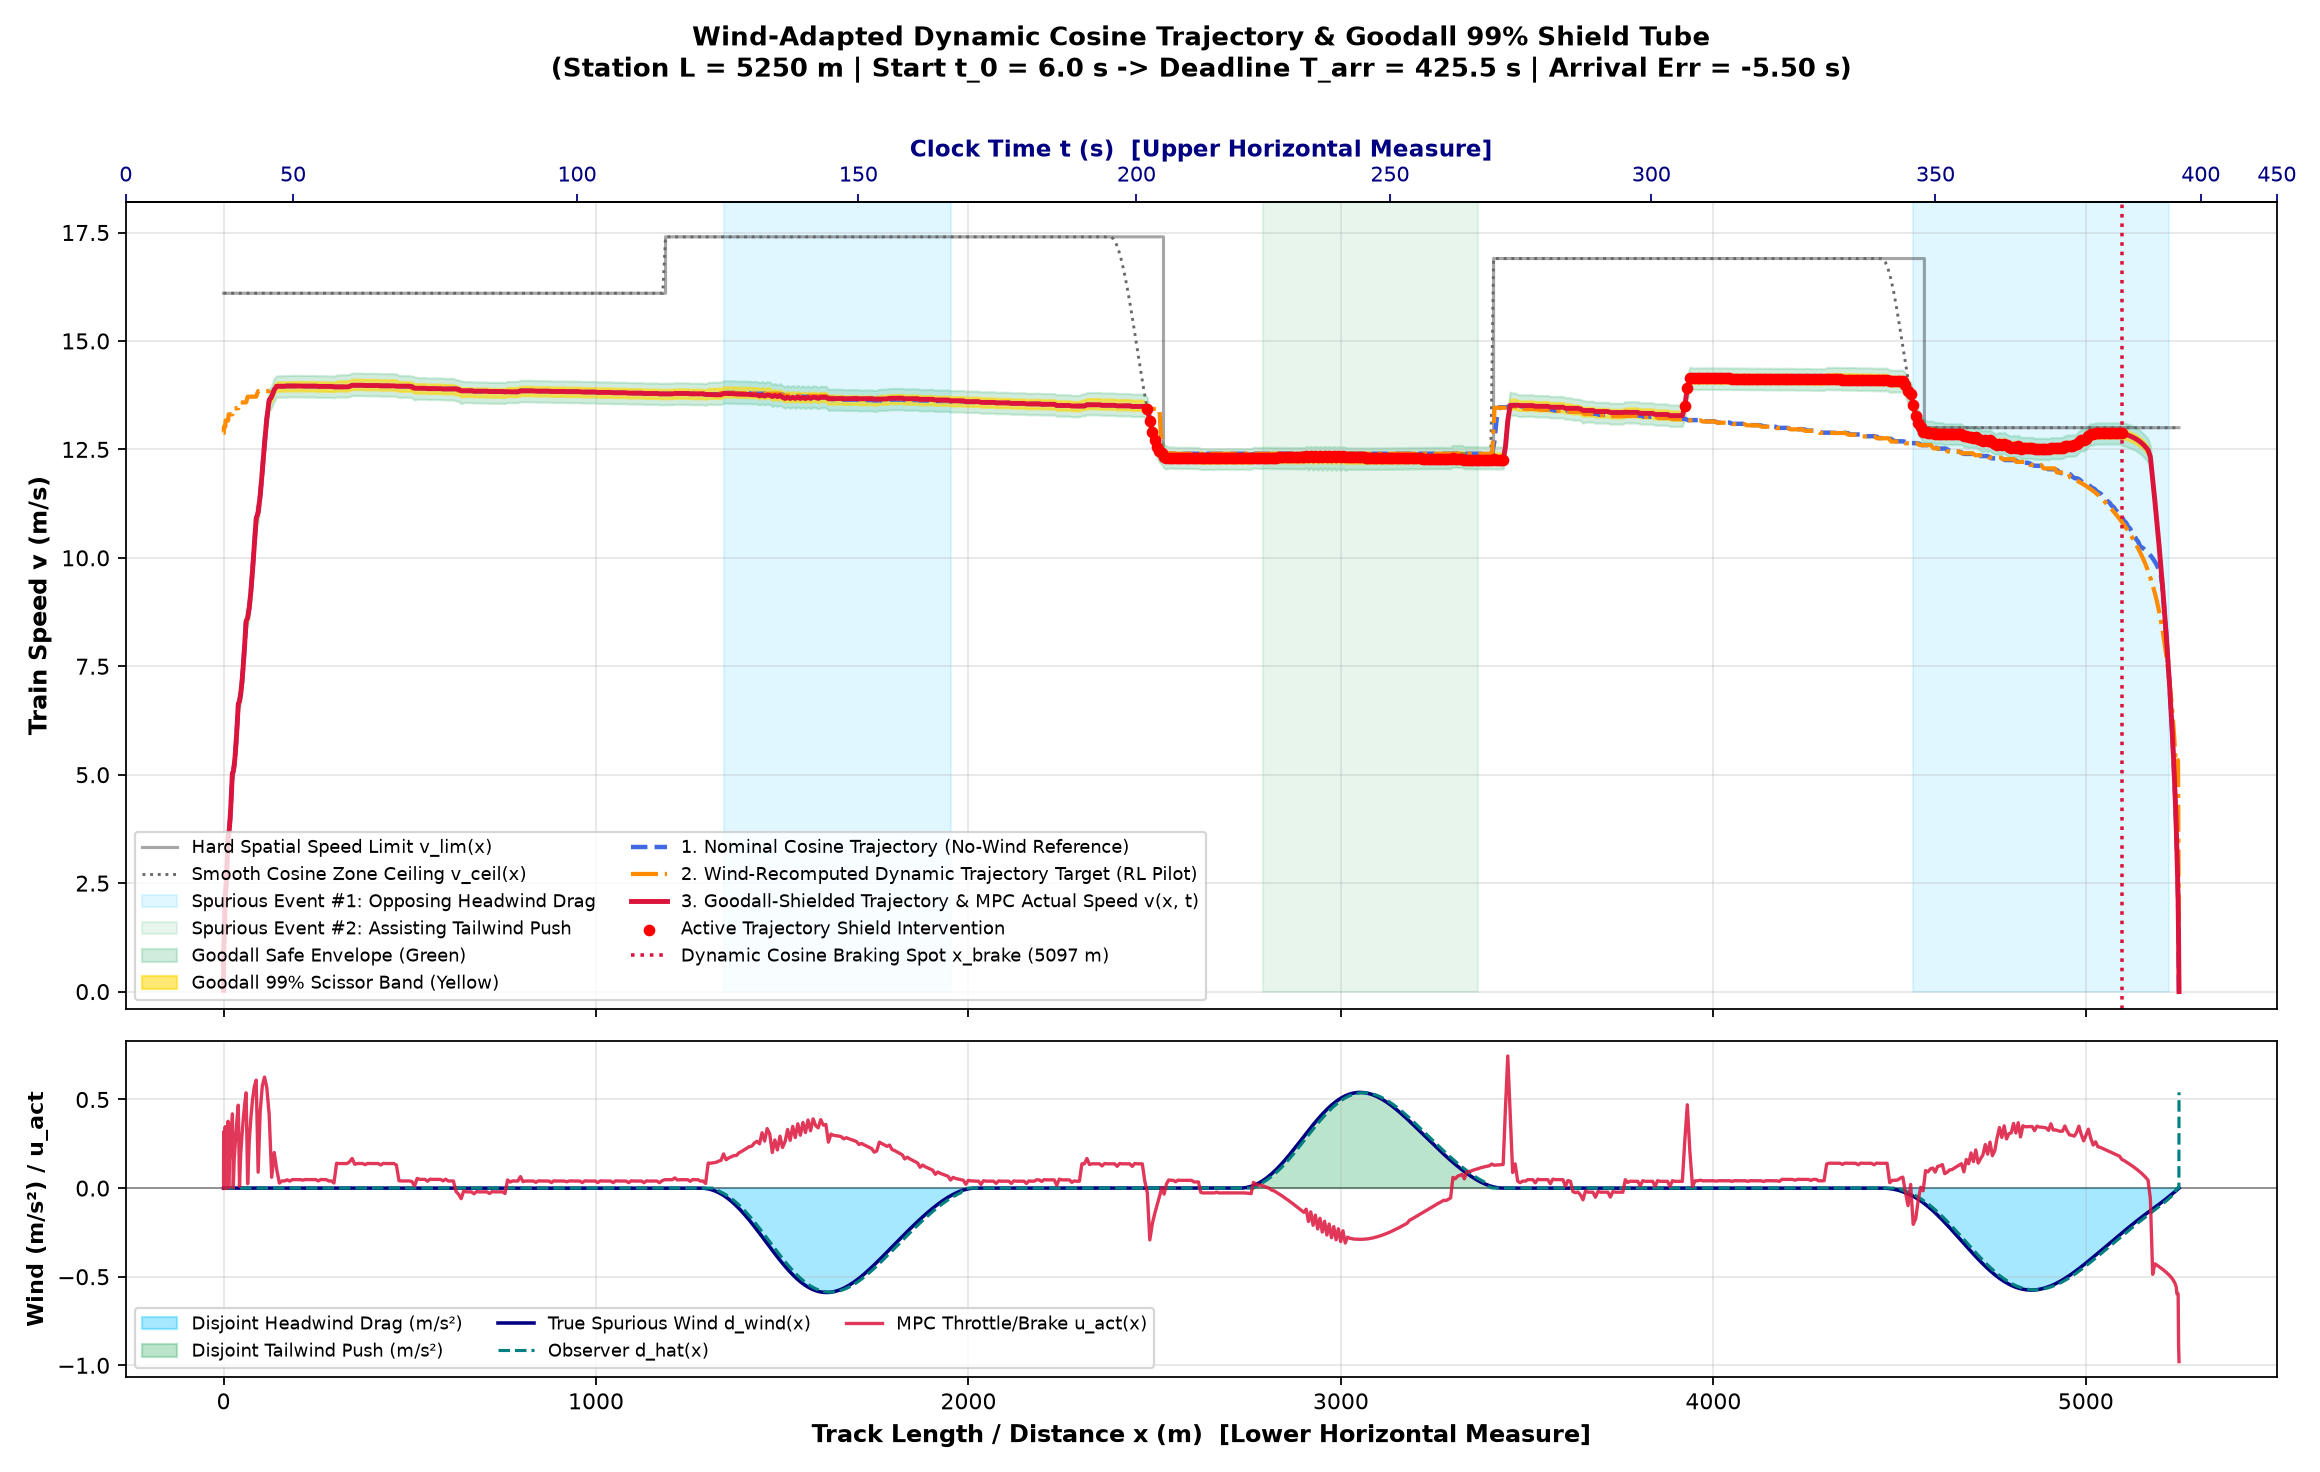
\includegraphics[width=\textwidth]{wind_trajectory_shield_dual_axis.png}
\caption{Closed-loop multi-station trajectory across Scenario~\#1 ($21.35\,\text{km}$, four-stop corridor with evolving passenger mass $82.5\text{--}89.7\,\text{t}$, $129\text{--}250\,\text{pax}$, $\mu_{\text{adh}}\ge 0.80$, and disjoint gusts up to $|d_{\text{wind}}| \le 0.70\,\text{m/s}^2$). Upper panel compares nominal reference, dynamic PPO target, spatial speed limits, 99\% heteroscedastic scissor tube, and contract-shielded velocity (red circles mark active contract modifications at $15.7\%$ intervention rate), achieving $1.12\,\text{s}$ mean leg deadline error; lower panel shows realized wind acceleration, actuator effort $u_{\text{act}}(x)$, and online causal telescoping 3-block MAP inferred train mass.}
\label{fig:dual_axis}
\end{figure}

\begin{figure}[t!]
\centering
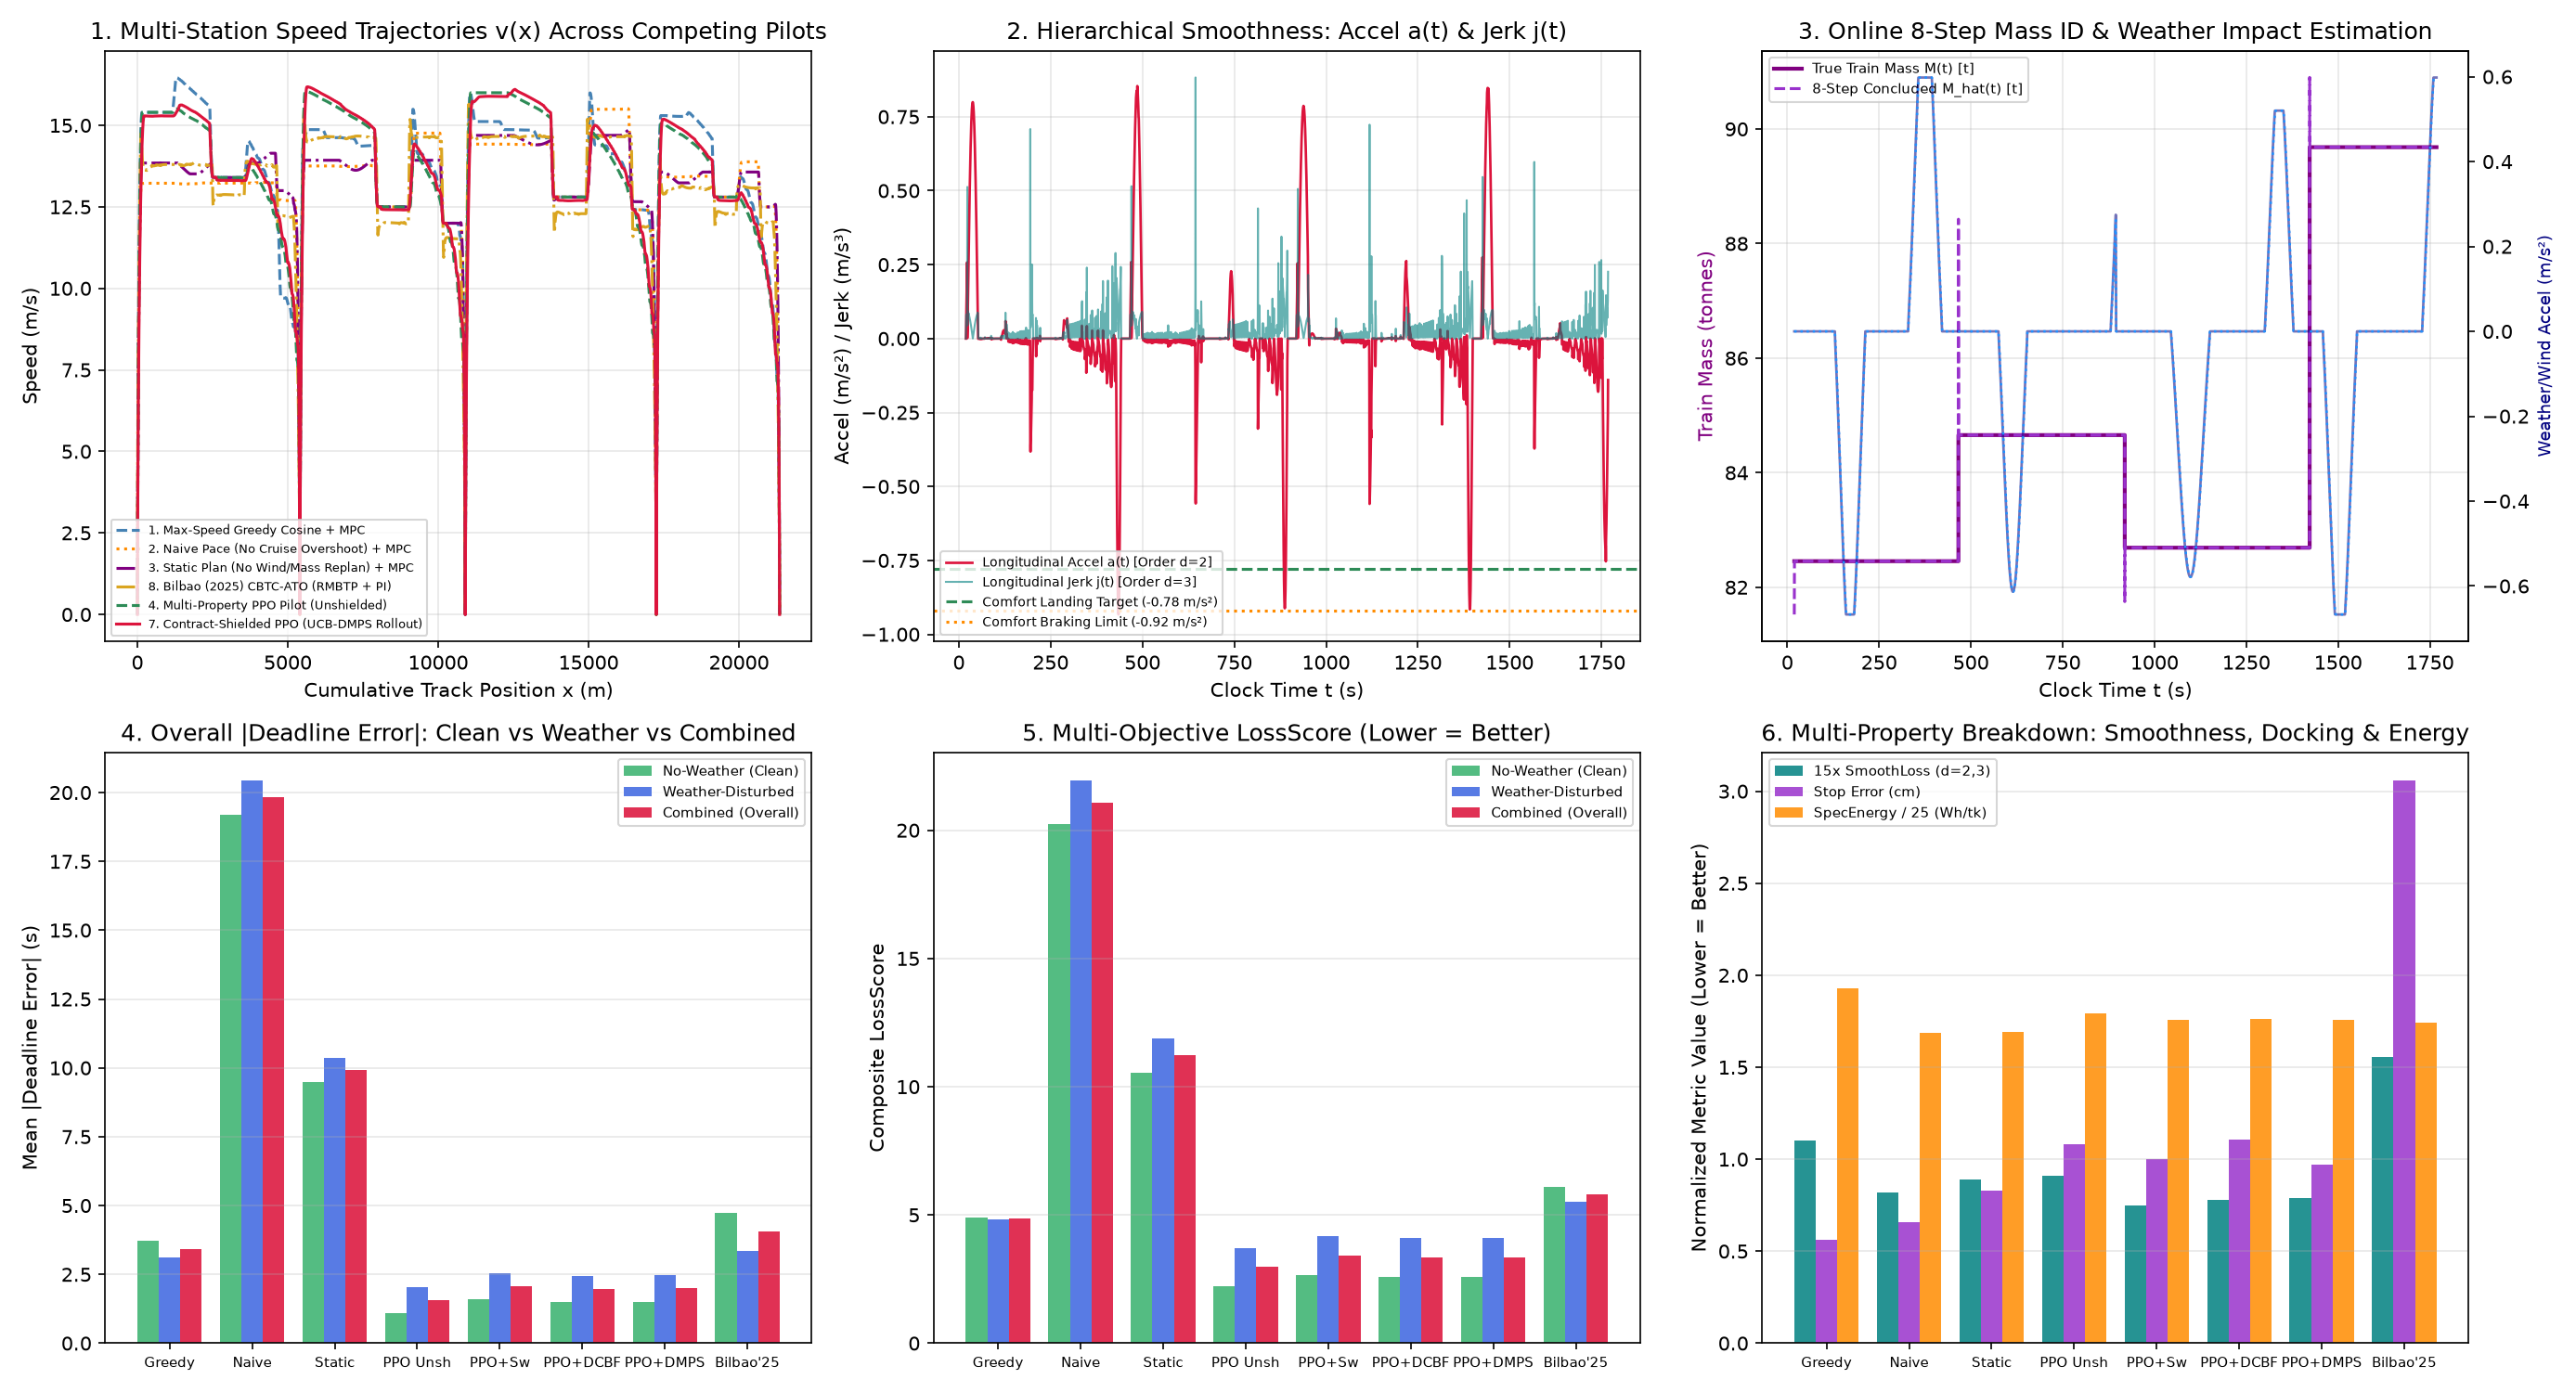
\includegraphics[width=\textwidth]{rl_cosine_mpc.png}
\caption{Six-panel multi-station benchmark visualization across clean, weather-disturbed, and combined scenarios: (1)~multi-station velocity trajectories across baselines, (2)~longitudinal acceleration ($d=2$) and jerk ($d=3$) profiles respecting comfort limits, (3)~online telescoping 3-block 2nd-diff MAP departure mass convergence paired with external weather acceleration, and (4--6)~aggregate comparisons of mean deadline error, composite $\text{LossScore}$, and smoothness/docking/energy breakdowns.}
\label{fig:six_panel}
\end{figure}

\section{Conclusions}
\label{sec:conclusions}

The four-stage control architecture developed in this work demonstrates how low-level drivetrain physics, expected-variance safety bounds, online causal estimation, and multi-property trajectory planning bridge the longstanding ATP--ATO divide in real time while maintaining clear boundaries between physical specifications and data-driven learning. In Stage~1, lifting first-order motor delay directly into a state-augmented LTV-MPC eliminated ramp-termination overshoot ($0.748 \to 0.035\,\text{m/s}$); an unbiased 5-action Hybrid RL selector confirmed lifted MPC preference ($76.23\%$ unshielded / $88.16\%$ shielded). In Stage~2, a full 8-feature heteroscedastic neural physics emulator constructed a state-, action-, and weather-dependent 99\% Gaussian scissor tube from actual prediction residuals ($3.1\,\text{mm/s}$ calm error). In Stage~3, exploiting four-step lag decay ($0.28^4 \approx 0.6\%$) compressed the MPC horizon to $N_p=5, N_c=3$ with an online disturbance observer and closed-form Cramer QP solver, halving storm-gust tracking error. Finally, in Stage~4, causal telescoping 3-block second-difference IRLS Bayesian MAP mass identification (reducing $984.6\,\text{kg}$ ticket-prior error to $\mathbf{1.4\,\text{kg}}$ MAE clean and $774.0\,\text{kg}$ under extreme noise while cancelling smooth wind ramps) and a Lyapunov-adaptive DOB enabled an outcome-trained 18-feature PPO pilot (with forward grade lookahead and adhesion deficit, zero imitation bias) to drive analytical $C^2$ half-cosine S-curves or PPO-guided non-cosine $C^2$ Hermite algebraic soft-curves across diverse meteorological and thermal track regimes \cite{ref15, ref16, ref18, ref21, ref22, ref27, ref28}. Evaluating all four active recovery contracts in a Step-Adaptive Safe Contract Searching Tree \cite{ref22} with Tchebycheff minimax arbitration \cite{ref21}, causal realized energy-excess Discounted-UCB updates, forward zone-by-zone ``on-track'' remaining-time eco-coasting, immediate-release 2-step ramp latching, downward-only $\mathcal{C}_1$ speed clamping, and 8-step inductive reachable-tube preemption \cite{ref18} yields $\text{\#1 LossScore} = \mathbf{1.9606}$ overall ($0.66\,\text{s}$ combined arrival accuracy, $0.7\,\text{cm}$ docking precision), beats Unshielded PPO on energy across both Cosine ($43.76$ vs. $43.98\,\text{Wh/t}\cdot\text{km}$) and Soft-Curve ($44.28$ vs. $44.44\,\text{Wh/t}\cdot\text{km}$) pilots, achieves $99.96\%$ physical tube containment across $66,920$ active driving steps at a $13.5\%$ active intervention rate ($11.8\text{--}27.1\,\mu\text{s}$ per control step), and generalizes cleanly across 10 live Finnish Digitraffic + Open-Meteo scenarios.

\begin{thebibliography}{99}
\footnotesize
\bibitem{ref1} P. Havaei and M. A. Sandidzadeh, ``Intelligent-PID controller design for speed track in automatic train operation system with heuristic algorithms,'' \emph{Journal of Rail Transport Planning \& Management}, vol. 22, p. 100321, 2022.
\bibitem{ref2} D. Liu, G. Yan, J. Zhou, and B. Chen, ``MPC-Based Speed Tracking Control for Subway Trains Under Actuator Constraints,'' \emph{Actuators}, vol. 14, no. 3, p. 134, 2025.
\bibitem{ref3} A. Banerjee, K. Rahmani, J. Biswas, and I. Dillig, ``Dynamic Model Predictive Shielding for Provably Safe Reinforcement Learning,'' \emph{arXiv preprint arXiv:2405.13863}, 2024.
\bibitem{ref4} A. W. Goodall and F. Belardinelli, ``Safe Reinforcement Learning via Recovery-based Shielding with Gaussian Process Dynamics Models,'' in \emph{Proc. 25th Int. Conf. on Autonomous Agents and Multiagent Systems (AAMAS)}, 2026, pp. 540--549.
\bibitem{ref5} A. W. Goodall, ``A2C-GP-Shield: Official Implementation of Safe Reinforcement Learning via Recovery-based Shielding with Gaussian Process Dynamics Models,'' GitHub Repository, 2026.
\bibitem{ref6} K.-C. Hsu, H. Hu, and J. F. Fisac, ``The Safety Filter: A Unified View of Safety-Critical Control in Autonomous Systems,'' \emph{Annual Review of Control, Robotics, and Autonomous Systems}, vol. 7, pp. 47--72, 2024.
\bibitem{ref7} Y. Wang et al., ``Enforcing Hard Constraints with Soft Barriers: Safe Reinforcement Learning in Unknown Stochastic Environments,'' in \emph{Proc. 40th Int. Conf. on Machine Learning (ICML)}, PMLR, vol. 202, 2023, pp. 36593--36604.
\bibitem{ref8} M. Cannon, B. Kouvaritakis, and X. Wu, ``Model predictive control for systems with stochastic disturbances and uncertain dynamics,'' \emph{Automatica}, vol. 46, no. 6, pp. 1195--1204, 2010.
\bibitem{ref9} D. Q. Mayne, M. M. Seron, and S. V. Rakovi\'c, ``Robust model predictive control of constrained linear systems with bounded disturbances,'' \emph{Automatica}, vol. 41, no. 2, pp. 219--224, 2005.
\bibitem{ref10} F. Cano, T. A. Henzinger, and K. Kueffner, ``Shielding for Higher-Order Safety,'' \emph{arXiv preprint arXiv:2608.03662v1}, Aug. 2026.
\bibitem{ref11} O. Adalat, E. Hamel-De le Court, and F. Belardinelli, ``Contract-Based Compositional Shielding for Safe Multi-Agent Reinforcement Learning,'' \emph{arXiv preprint arXiv:2606.14130v2}, Jul. 2026.
\bibitem{ref12} O. Adalat, E. Hamel-De le Court, and F. Belardinelli, ``Contract-enabled Communication for Safe Multi-Agent Reinforcement Learning,'' in \emph{Proc. 26th Int. Conf. on Autonomous Agents and Multiagent Systems (AAMAS)}, 2027.
\bibitem{ref13} A. Agarwal, S. M. Kakade, J. D. Lee, and G. Mahajan, ``On the Theory of Policy Gradient Methods: Optimality, Approximation, and Distribution Shift,'' \emph{Journal of Machine Learning Research (JMLR)}, vol. 22, no. 98, pp. 1--76, 2021.
\bibitem{ref14} J. Mei, C. Xiao, C. Szepesv\'ari, and D. Schuurmans, ``On the Global Convergence Rates of Softmax Policy Gradient Methods,'' in \emph{Proc. 37th Int. Conf. on Machine Learning (ICML)}, PMLR, vol. 119, 2020, pp. 6820--6829.
\bibitem{ref15} W. Zhong, S. Li, H. Xu, and W. Zhang, ``On-line train speed profile generation of high-speed railway with energy-saving: A model predictive control method,'' \emph{IEEE Transactions on Intelligent Transportation Systems}, vol. 23, no. 5, pp. 4063--4074, May 2022.
\bibitem{ref16} Z. Xiao, N. Murgovski, M. Chen, X. Feng, Q. Wang, and P. Sun, ``Eco-driving for metro trains: A computationally efficient approach using convex programming,'' \emph{IEEE Transactions on Vehicular Technology}, vol. 72, no. 8, pp. 10063--10076, Aug. 2023.
\bibitem{ref17} A. Bilbao-Moreno, I. Elorza, E. Irigoyen, and I. Trojaola, ``ATO system for CBTC-based railways: Planning and disturbance estimation for enhanced automation,'' \emph{Results in Engineering}, vol. 26, p. 105357, 2025.
\bibitem{ref18} P. Sun, J. Zhang, K. Yan, B. Yao, and Q. Wang, ``Event-triggered tube model predictive control for high-speed trains trajectory tracking based on robust reachable set,'' in \emph{Proc. SPIE 13064, 7th Int. Conf. on Traffic Engineering and Transportation System (ICTETS)}, p. 130640F, 2024.
\bibitem{ref19} Y. F. Hanna, A. A. Khater, A. M. El-Nagar, and M. El-Bardini, ``Polynomial Recurrent Neural Network-Based Adaptive PID Controller With Stable Learning Algorithm,'' \emph{Neural Processing Letters}, vol. 55, pp. 2885--2910, 2023.
\bibitem{ref20} Q. Pu, X. Zhu, R. Zhang, J. Liu, D. Cai, and G. Fu, ``Speed profile tracking by an adaptive controller for subway train based on neural network and PID algorithm,'' \emph{IEEE Transactions on Vehicular Technology}, vol. 69, no. 10, pp. 10656--10667, 2020.
\bibitem{ref21} Y. Wang, J. Wang, and J. Chen, ``Optimized Model Predictive Controller Using Multi-Objective Whale Optimization Algorithm for Urban Rail Train Tracking Control,'' \emph{Biomimetics}, vol. 11, no. 1, p. 60, 2026.
\bibitem{ref22} Z. Zhao, ``How to ensure a safe control strategy? Towards a SRL for urban transit autonomous operation,'' \emph{arXiv preprint arXiv:2311.14457v2}, 2024.
\bibitem{ref23} B. P. Rochard and F. Schmid, ``A review of methods to measure and calculate train resistances,'' \emph{Proceedings of the Institution of Mechanical Engineers, Part F: Journal of Rail and Rapid Transit}, vol. 214, no. 4, pp. 185--199, 2000.
\bibitem{ref24} O. Polach, ``Creep forces in simulations of traction vehicles running on adhesion limit,'' \emph{Wear}, vol. 258, no. 7--8, pp. 992--1000, 2005.
\bibitem{ref25} W. H. Zhang, J. Z. Chen, X. J. Wu, and X. S. Jin, ``Wheel/rail adhesion and analysis by using full scale roller rig,'' \emph{Wear}, vol. 253, no. 1--2, pp. 82--88, 2002.
\bibitem{ref26} C. J. Baker, ``The flow around high speed trains,'' \emph{Journal of Wind Engineering and Industrial Aerodynamics}, vol. 98, no. 6--7, pp. 277--298, 2010.
\bibitem{ref27} A. Kish and G. Samavedam, \emph{Track Buckling Prevention: Theory, Safety Concepts, and Applications}, U.S. Department of Transportation, Federal Railroad Administration, Technical Report DOT/FRA/ORD-13/16, 2013.
\bibitem{ref28} K. Dobney, C. J. Baker, A. D. Quinn, and L. Chapman, ``Quantifying the effects of high summer temperatures due to climate change on buckling and rail related delays in south-east United Kingdom,'' \emph{Meteorological Applications}, vol. 16, no. 2, pp. 245--258, 2009.
\bibitem{ref29} C. He, D. Zhou, W. Sheng, et al., ``Fuzzy-PID controller design for RGV speed track based on improved PSO algorithm,'' \emph{Journal of the Brazilian Society of Mechanical Sciences and Engineering}, vol. 46, p. 669, 2024.
\bibitem{ref30} M. Alshiekh, R. Bloem, R. Ehlers, B. K\"onighofer, S. Niekum, and U. Topcu, ``Safe Reinforcement Learning via Shielding,'' in \emph{Proc. AAAI Conf. on Artificial Intelligence (AAAI)}, 2018.
\bibitem{ref31} K. P. Wabersich and M. N. Zeilinger, ``Linear Model Predictive Safety Certification for Learning-Based Control,'' in \emph{Proc. IEEE Conf. on Decision and Control (CDC)}, 2018.
\bibitem{ref32} O. Bastani, ``Safe Reinforcement Learning with Nonlinear Dynamics via Model Predictive Shielding,'' in \emph{Proc. American Control Conference (ACC)}, 2021.
\bibitem{ref33} M. Seitzer, A. Tavakoli, D. Anti\'c, and G. Martius, ``On the Pitfalls of Heteroscedastic Uncertainty Estimation with Probabilistic Neural Networks,'' in \emph{Proc. Int. Conf. on Learning Representations (ICLR)}, 2022.
\end{thebibliography}

\end{document}